\chapter{\label{sec:lr:cpsystems}\glsentrytext{cps}: \glsentrytext{ps} with Complex Symbols}
\fxerror*{Expand/explain}{\cite{Nicolescu2014b,Nicolescu2017}}

\gls{cps} is another variant of \gls{ps}, developed by Nicolescu and collaborators in the early 2010s \fxerror[inline]{[ref]} and complementary to the classic trinity of \gls{clps} \cite{Paun2000}, \gls{tlps} \cite{Martin-Vide2003}, and \gls{snps} \cite{Ionescu2006}.  It is largely based on \gls{clps} in that the core unit of it is the \emph{\gls{tlc}}, which is arranged as a nested tree structure and arguably can be seen, to some extent at least, as a higher-level abstraction over \gls{clps} \cite{Nicolescu2018}.  It can also incorporate elements of \gls{tlps}, in that \gls{cps} includes concepts of channels and message passing between \glspl{tlc} \cite{Henderson2019}, with an arbitrary number of these cells in the environment.  

A key difference from \gls{clps} and \gls{tlps}, however, is that in \gls{cps} \emph{only} the \glspl{tlc} have accompanying rules.  All subcells are merely inert symbolic objects operated upon by the \gls{tlc}'s rules.  These subcells are represented as labelled multisets within the \glspl{tlc}.  \citeauthor{Nicolescu2014a} demonstrated that not only is \gls{cps} capable of performing the same tasks as other \gls{ps} variants, but it also can be used to model standard computer programs \cite{Nicolescu2014a}.

The principal advantage of \gls{cps} over traditional \gls{clps} is a simplification in the specification of complete systems to solve a given problem.  \Gls{clps} (as well as \gls{tlps} and \gls{snps}) typically require the definition of a uniform or semi-uniform family of rulesets customised to the specific instance of the problem at hand, whereas \gls{cps} normally requires only the definition of a fixed (usually much shorter) set of rules that cover all possible instances. As a result, only inputs to the system need to vary to solve different instances of the problem, e.g., in \cref{chap:tsp} just five fixed rules are necessary to solve any instance of the \gls{tsp}, requiring only customisation of the input objects (in that case, elements describing the nodes and edges of the graph).

This \namecref{sec:lr:cpsystems} provides an overview of \gls{cps}.  Further presentation of \gls{cps} has appeared most recently in \cite{Nicolescu2018,Henderson2019,Henderson2020,Liu2020,Liu2021}, and it is recommended that the interested reader peruse those too.  While \gls{cps} is transitively bio-inspired through its basis in \gls{ps}, it has not been developed to simulate or model real-world biology.  Instead, it is intended as a useful theoretical model for computation.

\begin{anfxwarning}
Really need to include a formal BNF grammar somewhere in here.
\end{anfxwarning}

% --------------------------------------------------

%-----------------------------------------------------------------------------------
\section{\label{sec:cps:complexsymbols}Complex Symbols as Subcells}
%-----------------------------------------------------------------------------------

\emph{Complex symbols} or \emph{subcells}, 
play the roles of cellular microcompartments or substructures,
such as organelles, vesicles, or cytoophidium assemblies (``snakes''),
which are embedded in cells or travel between cells, 
but without having the full processing power of a complete cell.
In \gls{cps}, subcells represent nested, labelled, data-only \glspl{compartment}
with no processing power of their own;
instead, the rules of their enclosing cells act upon them.
% instead, they are acted upon by the rules of their enclosing cells.

% Subcells can be either \emph{atoms} or \emph{compound terms}: multisets labelled by \emph{\glspl{functor}} (`\gls{functor}' is also commonly used as a shorthand for said compound terms).  Atoms, as the name suggests, are indivisible symbols.  They can be of any given type relevant to a system, but are static objects with no other inherent distinctive properties.  Atoms are written simply as the name of the atom's type.  Compound terms are objects that may contain both atoms and other compound terms and are written with the \gls{functor}'s type, followed by opening and closing parentheses, surrounding the encapsulated multiset.\footnote{For legibility, many compound terms in this work have been written with growing parentheses, dependent upon the level of nesting of terms involved.  This typesetting behaviour is not required or even specified as a part of \gls{cps} and can be freely omitted.}

%-------------------------------------------------------
\subsection{\label{sec:cps:terms}Subcells' Symbols} 
%-------------------------------------------------------

Subcells can be either \emph{atoms} or \emph{compound terms}: multisets labelled by \emph{\glspl{functor}} (`\gls{functor}' is also commonly used as a shorthand for said compound terms).  Atoms, as the name suggests, are indivisible symbols.  They can be of any given type relevant to a system, but are static objects with no other inherent distinctive properties.  Atoms are written simply as the name of the atom's type.  Compound terms are objects that may contain both atoms and other compound terms and are written with the \gls{functor}'s type, followed by opening and closing parentheses, surrounding the encapsulated multiset.\footnote{For legibility, many compound terms in this work have been written with growing parentheses, dependent upon the level of nesting of terms involved.  This typesetting behaviour is not required or even specified as a part of \gls{cps} and can be freely omitted.}

The basic vocabulary consists of atoms and \emph{variables}, collectively known as \emph{simple symbols}.  \emph{Complex symbols} are similar to Prolog-like \emph{first-order terms}, recursively built from \emph{multisets} of atoms and variables.  Together, complex symbols and simple symbols (atoms, variables) are called \emph{symbols} and can be defined by the following formal grammar:

\begin{framed}
\vspace{-0.6cm}
\begin{small}
\begin{bnf*}
    \bnfprod*{symbol}{\bnfpn{atom} \bnfor \bnfpn{variable} \bnfor \bnfpn{term}}\\
    \bnfprod*{term}{\bnfpn{functor} \bnfsp \bnfts{`('} \bnfsp \bnfpn{argument} \bnfsp \bnfts{`)'}}\\
    \bnfprod*{functor}{\bnfpn{atom}}\\
    \bnfprod*{argument}{\bnfes \bnfor \bnfsp \bnfpn{symbol} \bnfsp \bnfts{+}}
\end{bnf*}
\end{small}
\vspace{-0.8cm}
\end{framed}

Atoms are typically denoted by lower case letters (or, occasionally, digits), usually drawn from the Latin alphabet, 
such as \(a\), \(b\), \(c\), \(\cpundig\). 
Variables are typically denoted by upper case letters, 
such as \(X\), \(Y\), \(Z\).
\Eg{} an x atom may be written as \(x\), while a compound term labelled by a y \gls{functor} might be written as \(\cpfunc{y}{a \, xx \, z}\).  When there is more than one of a given atom present, the count is usually written as a superscript, so the earlier compound term would look like \(\cpfunc{y}{a \, x^2 \, z}\).  
\Glspl{functor} can only be atoms, not variables.

While not strictly necessary, one may also use \emph{anonymous variables} for improved readability, denoted by underscores (``\(\cpdiscard\)'').
Each underscore occurrence represents a \emph{new} unnamed variable
and indicates that something must fill that slot, but the specifics of what are unimportant.

Symbols that do \emph{not} contain variables are called \emph{ground}, \eg{}:
\begin{itemize}
\item Ground symbols:
\(a\), \(\cpfunc{a}{\cpempty}\), \(\cpfunc{a}{b}\), \(\cpfunc{a}{b c}\), \(\cpfunc{a}{b^2 c}\), \(\cpfunc{a}{\cpfunc{b}{c}}\), \(\cpfunc{a}{b\cpfunc{c}{\cpempty}}\), \(\cpfunc{a}{\cpfunc{b}{c}\cpfunc{d}{e}}\), \(\cpfunc{a}{\cpfunc{b}{c}\cpfunc{d}{e}}\), \(\cpfunc{a}{\cpfunc{b}{c}\cpfunc{d}{\cpfunc{e}{\cpempty}}}\), \(\cpfunc{a}{bc^2 d}\).

\smallskip
\item Symbols which are not ground:
\(X\), \(\cpfunc{a}{X}\), \(\cpfunc{a}{bX}\), \(\cpfunc{a}{\cpfunc{b}{X}}\), \(\cpfunc{a}{XY}\), \(\cpfunc{a}{X^2}\), \(\cpfunc{a}{XdY}\),  \(\cpfunc{a}{X\cpfunc{c}{}}\), \(\cpfunc{a}{\cpfunc{b}{X}\cpfunc{d}{e}}\), \(\cpfunc{a}{\cpfunc{b}{c}\cpfunc{d}{Y}}\), \(\cpfunc{a}{\cpfunc{b}{X^2}\cpfunc{d}{\cpfunc{e}{Xf^2}}}\);
also, using anonymous variables: \(\_\), \(\cpfunc{a}{b\_}\), \(\cpfunc{a}{X\_}\), \(\cpfunc{a}{\cpfunc{b}{X}\cpfunc{d}{\cpfunc{e}{\_}}}\).

\smallskip
\item This term-like construct which starts with a variable is \emph{not} a symbol (the above grammar defines first-order terms only):
\(\cpfunc{X}{a Y}\).
\end{itemize}

In \emph{concrete} models, cells contain ground symbols only.
Rules may, however, contain \emph{any} kind of symbols, atoms, variables, and terms (whether ground or not).

%-------------------------------------------------------
\subsection{\label{sec:cps:specialpurposeatoms}Special-purpose Atoms} 
%-------------------------------------------------------

There are two special atoms defined with specific meanings across \gls{cps}.  Empty multisets are denoted with \(\cpempty\), and instances of natural numbers with the \emph{counting atom} (see further \vref{sec:cps:natnums}).
One may abbreviate the expression of complex symbols by removing inner \(\cpempty\)'s as explicit references to the empty multiset, \eg{}~\(\cpfunc{a}{\cpempty} = \cpfunc{a}{\,}\).  Alternatively, where the term stores a number, \(\cpempty\) may instead be replaced with \(0\) (\ie{} the numeral for zero).

%-------------------------------------------------------
\subsection{\label{sec:cps:unification}Unification} 
%-------------------------------------------------------
All symbols which appear in rules (ground or not) can be (asymmetrically) \emph{matched} against \emph{ground} terms,
using an ad-hoc version of \emph{pattern matching}, 
more precisely, a \emph{one-way first-order syntactic unification} (one-way, because \glspl{tlc} may not contain variables) \cite{Liu2021}.
An atom can only match another copy of itself, but
a variable can match any multiset of ground terms (including \(\cpempty\)).
This may create combinatorial \emph{non-determinism}, 
when a combination of two or more variables are matched against the same multiset,
in which case an arbitrary matching is chosen. 
For example:
\begin{itemize}
\item Matching \(\cpfunc{a}{\cpfunc{b}{X}fY} = \cpfunc{a}{\cpfunc{b}{c\cpfunc{d}{e}}f^2g}\) deterministically creates a single set of unifiers:
\(X, Y = c\cpfunc{d}{e}, fg\).

\smallskip
\item Matching \(\cpfunc{a}{XY^2} = \cpfunc{a}{de^2f}\) deterministically creates a single set of unifiers: 
\(X, Y = df, e\).

\smallskip
\item Matching \(\cpfunc{a}{\cpfunc{b}{X}\cpfunc{c}{\cpundig X}} = \cpfunc{a}{\cpfunc{b}{\cpundig^2}\cpfunc{c}{\cpundig^3}}\) deterministically creates one single unifier: 
\(X = \cpundig^2\).

\smallskip
\item Matching \(\cpfunc{a}{\cpfunc{b}{X}\cpfunc{c}{\cpundig X}} = \cpfunc{a}{\cpfunc{b}{\cpundig^2}\cpfunc{c}{\cpundig^2}}\) fails.

\smallskip
\item Matching \(\cpfunc{a}{XY} = \cpfunc{a}{df}\) non-deterministically creates one of the following four sets of unifiers: 
\(X, Y = \cpempty, df\); \(X, Y = df, \cpempty\); \(X, Y = d, f\); \(X, Y = f, d\). 
\end{itemize}

% %-----------------------------------------
% \subsubsection{Performance Note}
% %-----------------------------------------
% If the rules avoid any matching non-determinism, 
% this proposal should not affect the performance of \gls{ps} simulators running on existing machines.
% Assuming that multisets/bags are already taken care of, \eg{}~via hash-tables,
% the proposed unification probably adds an almost linear factor.
% Recall that, in similar contexts (no occurs check needed), 
% Prolog unification algorithms can run in \(O(n g(n))\) steps,
% where \(g\) is the inverse Ackermann function.
% This conjecture must be proven, though, 
% as the novel presence of multisets may affect the performance.

% % -------------------------------------------------
%-----------------------------------------------------------------------------------
\section{\label{sec:cps:highlevelrules}High-level or Generic Rules}
%-----------------------------------------------------------------------------------

%-------------------------------------------------------
\subsection{\label{sec:cps:genericrules}Generic Rules Format}
%-------------------------------------------------------
% Consider rules of the following \emph{generic} format 
% (called generic because it defines templates involving variables):
% \begin{framed}
% \vspace{-0.6cm}
% \begin{align*}
% \textsf{current-state} ~~ \textsf{symbols} \dots ~ \rightarrow_\alpha ~ & \textsf{target-state} ~~ (\textsf{in-symbols}) \dots ~~ \\
%  & (\textsf{out-symbols})_\delta \dots \\
%  & | ~  \textsf{\glspl{promoter}} \dots ~~ \neg ~  \textsf{\glspl{inhibitor}} \dots
% \end{align*}
% \vspace{-0.8cm}
% \end{framed}
% Where:
% \begin{itemize}
% \item \textsf{current-state} and \textsf{target-state} are atoms or terms;  these are traditionally written in the form \(s_x\) where \(x\) is a sequential numeral (\eg{} \(s_1\), \(s_2\) \etc{}), but any valid ground atom or term as appropriate is permitted.

% \smallskip
% \item \textsf{symbols}, \textsf{in-symbols}, \textsf{\glspl{promoter}} and \textsf{\glspl{inhibitor}} are symbols;

% \smallskip
% \item \textsf{in-symbols} become available after the end of the current step only, as in traditional \gls{ps}  (one can imagine that these are sent via an \adhoc{} fast \textsf{loopback} channel); 

% \smallskip
% \item subscript \(\alpha\) \(\in\) \(\{\cponce\), \(\cpmaxpar\}\), 
% indicates the application mode, discussed further in \cref{sec:cps:applicationmodes};

% \smallskip
% \item \textsf{out-symbols} are sent to the cell's structural neighbours at the end of the step.
% These symbols are enclosed in angle brackets that indicate 
% their destinations, abbreviated above as \(\delta\). 
% The most usual scenarios include: 

% \begin{itemize}
% \item \(\cpoutsymbol{a}{i}\) indicates that \(a\) is sent over outgoing arc \(i\) (unicast); 

% \item \(\cpoutsymbol{a}{i,j}\) indicates that \(a\) is sent over outgoing arcs \(i\) and \(j\)(multicast); 

% \item \(\cpoutsymbolall{a}\) indicates that \(a\) is sent over all outgoing arcs (broadcast). 
% \end{itemize}

% All symbols sent via one \emph{generic rule} to the same destination form one single \emph{message}, and they travel together as one single block (even if the generic rule is applied in mode \(\cpmaxpar\)).
% \end{itemize}

Consider rules of the following \emph{generic} format 
(called generic because it defines templates involving variables):
\begin{framed}
\vspace{-0.6cm}
\begin{align*}
 current-state  ~~  symbols  \dots ~ \rightarrow_\alpha ~ &  target-state  ~~ ( in-symbols ) \dots ~~ \\
 & | ~  \glspl{promoter} \dots ~~ \neg ~  \glspl{inhibitor} \dots
\end{align*}
\vspace{-0.8cm}
\end{framed}
Where:
\begin{itemize}
\item  current-state  and  target-state  are atoms or terms;  these are traditionally written in the form \(s_x\) where \(x\) is a sequential numeral (\eg{} \(s_1\), \(s_2\) \etc{}), but any valid ground atom or term as appropriate is permitted.

\smallskip
\item  symbols, \glspl{promoter} and \glspl{inhibitor} are symbols;

\smallskip
\item  in-symbols  become available after the end of the current step only, as in traditional \gls{ps}  (one can imagine that these are sent via an \adhoc{} fast  loopback  channel); 

\smallskip
\item subscript \(\alpha\), \(\{\cponce\), \(\cpmaxpar\}\), 
indicates the application mode, discussed further in \cref{sec:cps:applicationmodes};

% \smallskip
% \item \textsf{out-symbols} are sent to the cell's structural neighbours at the end of the step.
% These symbols are enclosed in angle brackets that indicate 
% their destinations, abbreviated above as \(\delta\). 
% The most usual scenarios include: 

% \begin{itemize}
% \item \(\cpoutsymbol{a}{i}\) indicates that \(a\) is sent over outgoing arc \(i\) (unicast); 

% \item \(\cpoutsymbol{a}{i,j}\) indicates that \(a\) is sent over outgoing arcs \(i\) and \(j\)(multicast); 

% \item \(\cpoutsymbolall{a}\) indicates that \(a\) is sent over all outgoing arcs (broadcast). 
% \end{itemize}

% All symbols sent via one \emph{generic rule} to the same destination form one single \emph{message}, and they travel together as one single block (even if the generic rule is applied in mode \(\cpmaxpar\)).
\end{itemize}

%-------------------------------------------------------
\subsection{Pattern Matching}
%-------------------------------------------------------
Rules are matched against \gls{tlc} contents using the aforementioned \emph{pattern matching},
which involves the rule's \emph{\gls{lhs}}, \glspl{promoter} and \glspl{inhibitor}.

Generally, variables have \emph{global rule scope};
these are assumed to be introduced by \emph{existential} quantifiers preceding the rule
--- except for \glspl{inhibitor}, which may introduce \emph{local variables}, 
as further discussed in \vref{sec:cps:prominhi}. 

The matching is \emph{valid} only if, after unification/substituting variables by their values, 
the rule's \emph{\gls{rhs}} contains ground terms only
(so \emph{no} free variables are injected in the \gls{tlc} or sent to its neighbours),
as illustrated by the following sample scenario:
\begin{itemize}
\item The cell's \emph{current content} includes the \emph{ground term}:\\
\(\cpfunc{n}{a \, \cpfunc{\phi}{b \, \cpfunc{\phi}{c} \, \cpfunc{\psi}{d}} \, \cpfunc{\psi}{e}}\)

\smallskip
\item The following (state-less) \emph{rewriting rule} is considered: \\ 
\(\cpfunc{n}{X \, \cpfunc{\phi}{Y \, \cpfunc{\phi}{Y_1} \, \cpfunc{\psi}{Y_2}} \, \cpfunc{\psi}{Z}} ~ \rightarrow ~ \cpfunc{v}{X} \: \cpfunc{n}{Y \, \cpfunc{\phi}{Y_2} \, \cpfunc{\psi}{Y_1}} \: \cpfunc{v}{Z}\)

\smallskip
\item The pattern matching determines the following \emph{unifiers}: \\
\(X = a\), \(Y = b\), \(Y_1 = c\), \( Y_2 = d\), \(Z = e\).

\smallskip
\item This is a \emph{valid} matching and, after \emph{substitutions}, 
the rule's \gls{rhs} gives the \emph{new content}: \\
\(\cpfunc{v}{a} ~ \cpfunc{n}{b \, \cpfunc{\phi}{d} \, \cpfunc{\psi}{c}} ~ \cpfunc{v}{e}\)
\end{itemize}

%-------------------------------------------------------
\subsection{\label{sec:cps:prominhi}Promoters and Inhibitors}
%-------------------------------------------------------

Promoters are objects that \emph{must} be present within the \gls{tlc} for the rule to be applicable but are \emph{not} removed by the rule.  Conversely, \glspl{inhibitor} are objects that \emph{must not} be present for the rule to be applicable, although the rule may create them.  If \glspl{promoter} are present, they are denoted following a \(|\) per \gls{promoter}, and \glspl{inhibitor} by \(\neg\), \eg{} \(|\,\cpfunc{a}{A}\) or \(\neg\,\cpfunc{b}{B}\).  Promoters and \glspl{inhibitor} are traditionally written below the main rule body, but this is not strictly required.  Promoters are typically written first, followed by \glspl{inhibitor}, but this too is not compulsory.  All \glspl{promoter} and \glspl{inhibitor} have equal priority among themselves for a given attempted unification of a rule.

\lstset{xleftmargin=.5in, xrightmargin=.5in} 
\begin{lstlisting}
  $| ~ \cpfunc{a}{A}$ #\hfill \gls{promoter} \enspace#
  $\neg ~ \cpfunc{b}{B}$ #\hfill \gls{inhibitor} \enspace#
\end{lstlisting}

To define additional useful matchings expressively, 
\glspl{promoter} and \glspl{inhibitor} may also use virtual ``equality'' terms, 
written in infix format, with the \(=\) operator.
For example, including the term \((ab = XY)\) indicates the following additional matching constraints on variables \(X\) and \(Y\): either \(X, Y = ab, \cpempty\); or \(X, Y = a, b\); or \(X, Y = b, a\); or \(X, Y = \cpempty, ab\).

To define \glspl{inhibitor} as logical negations usefully,
variables that only appear in the scope of an \gls{inhibitor} are assumed to have \emph{local scope}. 
Furthermore, these variables are assumed to be defined by \emph{existential} quantifiers, immediately after the negation. 
Semantically, this is equivalent to introducing these variables at the global rule level, 
but by \emph{universal} quantifiers, after all other global variables;
introduced by \emph{existential} quantifiers.

As an illustration, consider a \gls{tlc} containing \(\cpfunc{a}{c} ~ \cpfunc{a}{ccc}\) and contrast two rules, 
containing the following two sample \gls{promoter}/\gls{inhibitor} pairs 
(for brevity, other rule details are omitted here).

\lstset{xleftmargin=.5in, xrightmargin=.5in} 
\begin{lstlisting}
... $\mid$  $\cpfunc{a}{cXY}$     $\neg$  $\cpfunc{a}{X}$    #\hfill (1)\enspace#
... $\mid$  $\cpfunc{a}{cZ}$     $\neg$  $(Z=XY)$  $\cpfunc{a}{X}$    #\hfill (2)\enspace#
\end{lstlisting}

These two rules appear very similar, and their \gls{inhibitor} tests share the same expression: 
\emph{No} \(\cpfunc{a}{X}\) may be present in the \gls{tlc}.

Rule (1) uses two global variables, \(X, Y\). 
According to its \gls{promoter}, \(\cpfunc{a}{cXY}\), these variables can be matched in four different ways:
(1a) \(X, Y = \cpempty, \cpempty\); (1b) \(X, Y = cc, \cpempty\); (1c) \(X, Y = \cpempty, cc\); (1d) \(X, Y = c, c\).\footnote{Strictly speaking, this matching is possible in multiple ways, with different \(c\) atoms assigned to each variable.  For current purposes, though, they are equivalent and so are reduced to the one result.}
Three different unifications, (1a), (1b), (1c), pass the \gls{inhibitor} test, 
as there are no cell terms \(\cpfunc{a}{\,}\), \(\cpfunc{a}{cc}\), \(\cpfunc{a}{\,}\), respectively. 
Unification (1d) fails the \gls{inhibitor} test because there \emph{is} one cell term \(\cpfunc{a}{c}\).

Rule (2) uses one global variable, \(Z\), and two local \gls{inhibitor} variables, \(X, Y\).
According to its \gls{promoter}, \(\cpfunc{a}{cZ}\), variable \(Z\) can be matched in two different ways: 
(2a) \(Z = \cpempty\); (2b) \(Z = cc\).
Unification (2a) passes the \gls{inhibitor} test because it only generates one local unification,
\(X, Y = \cpempty, \cpempty\), and there is \emph{no} cell term \(\cpfunc{a}{\,}\).
Unification (2b) fails the \gls{inhibitor} test because it generates all three following local unifications:
(2b1) \(X, Y = cc, \cpempty\); (2b2) \(X, Y = \cpempty, cc\); (2b3) \(X, Y = c, c\); 
and there \emph{is} a cell term corresponding to (2b3), \(\cpfunc{a}{c}\).

%-------------------------------------------------------
\subsection{\label{sec:cps:applicationmodes}Application Modes: Exactly-once and Maximally-parallel}
%-------------------------------------------------------
To explain the two rule application modes, \(\cponce\) and \(\cpmaxpar\) (referred to as \emph{exactly-once} and \emph{maximally-parallel} respectively) consider a \gls{tlc}, \(\sigma\), containing three counter-like complex symbols,
\(\cpfunc{c}{\cpundig^2}\), \(\cpfunc{c}{\cpundig^2}\), \(\cpfunc{c}{\cpundig^3}\),
and the two possible application modes of the following high-level ``decrementing'' rule:
\vspace{-0.2cm}
\begin{framed}
\vspace{-0.5cm}
\[(\rho_\beta) ~s_1 ~\cpfunc{c}{\cpundig \, X} \rightarrow_{\alpha} s_2 ~\cpfunc{c}{X},\\
\mathrm{where} \; \alpha \in \{\cponce, \cpmaxpar\}.\]
\vspace{-0.8cm}
\end{framed}

% The \gls{lhs} of rule \(\rho_\beta\), \(\cpfunc{c}{\cpundig \, X}\), can be unified in three different ways,
% to each one of the three \(c\) symbols extant in cell \(\sigma\).
% Conceptually, this rule may be instantiated in three different ways,
% each one tied and applicable to a distinct symbol:
Conceptually, the \gls{lhs} of rule \(\rho_\beta\), \(\cpfunc{c}{\cpundig \, X}\), can be unified in three different ways,
to each one of the three distinct \(c\) compound symbols extant in \gls{tlc} \(\sigma\):
% Conceptually, this rule may be instantiated in three different ways,
% each one tied and applicable to a distinct symbol:
\begin{eqnarray*}
& (\rho_1)  & ~s_1 ~\cpfunc{c}{\cpundig^2} \rightarrow_{\alpha} s_2 ~\cpfunc{c}{\cpundig},\\
& (\rho_2)  & ~s_1 ~\cpfunc{c}{\cpundig^2} \rightarrow_{\alpha} s_2 ~\cpfunc{c}{\cpundig},\\
& (\rho_3) & ~s_1 ~\cpfunc{c}{\cpundig^3} \rightarrow_{\alpha} s_2 ~\cpfunc{c}{\cpundig^2}.
\end{eqnarray*}

\begin{enumerate}
\item If \(\alpha = \: \cponce\), rule~\(\rho_1\) 
non-deterministically selects and applies one of these virtual rules \(\rho_1\), \(\rho_2\), \(\rho_3\).
Using \(\rho_1\) or \(\rho_2\), 
cell \(\sigma\) ends with counters \(\cpfunc{c}{\cpundig}\), \(\cpfunc{c}{\cpundig^2}\), \(\cpfunc{c}{\cpundig^3}\).
Using \(\rho_3\),
cell \(\sigma\) ends with counters \(\cpfunc{c}{\cpundig^2}\), \(\cpfunc{c}{\cpundig^2}\), \(\cpfunc{c}{\cpundig^2}\).

\smallskip
\item If \(\alpha = \: \cpmaxpar\), rule~\(\rho_\cpmaxpar\) 
applies in parallel all these virtual rules \(\rho_1\), \(\rho_2\), \(\rho_3\).
Cell \(\sigma\) ends with counters \(\cpfunc{c}{\cpundig}\), \(\cpfunc{c}{\cpundig}\), \(\cpfunc{c}{\cpundig^2}\).
\end{enumerate}

Semantically, the \(\cpmaxpar\) mode is equivalent to a virtual sequential \texttt{while} loop around the same rule in \(\cponce\) mode, which is repeated until it is no longer applicable.  All such applications of the rule are carried out concurrently in a single step, however.

Like most other \gls{ps} variants, \gls{cps} ordinarily evolve synchronously in a stepwise fashion following an implicit global clock.  Rules are applied based on whether the available multiset(s) within the system match the rules' \gls{lhs} and \glspl{promoter}, and not the \glspl{inhibitor}.  The consumption of removed objects plus the creation of new objects happens instantaneously at the end of a step.

%-------------------------------------------------------
\subsection{Benefits}
%-------------------------------------------------------
This type of generic rules allows
\begin{inparaenum}[(i)]
\item a reasonably fast parsing and processing of subcomponents; and
\item algorithm descriptions with \emph{fixed-size alphabets} and \emph{fixed-sized \glspl{ruleset}}, 
independent of the size of the problem and the number of \glspl{tlc} in the system (often \emph{impossible} with only atomic symbols).
\end{inparaenum}

%-------------------------------------------------------
\subsection{Special Cases}
%-------------------------------------------------------
Simple scenarios involving generic rules are sometimes 
semantically equivalent to sets of non-generic (ground) rules defined via bounded loops.
For example, consider the rule
\[
s_1 ~ \cpfunc{a}{IJ} ~ \rightarrow_\cpmaxpar ~ s_2 ~ \cpfunc{b}{I} ~ \cpfunc{c}{J},
\]
where the \gls{tlc}'s contents guarantee that \(I\) and \(J\) 
only match integers in ranges \([1,n]\) and \([1,m]\), respectively.
Under these assumptions, 
this rule is equivalent to the following set of non-generic rules:
\[
s_1 ~ a_{i,j} ~ \rightarrow s_2 ~ b_i ~ c_j, ~ \forall i \in [1,n], j \in [1,m].
\]

However, unification is a much more powerful concept, 
which cannot be reduced generally to simple bounded loops.
%-----------------------------------------------------------------------------------
\section{\label{sec:cps:formaldescriptions}Formal \glsfmtname{cps} Descriptions}
%-----------------------------------------------------------------------------------

A specific \glspl{cps} can be described by a 6-tuple, as shown below.

\[
\Pi_{cP}(T, A, O, R, S, \bar{s})
\]

\(T\) is the set of \glspl{tlc} at the start of the evolution of the system; \(A\) is the alphabet of the system; \(O\) is the set of multisets of initial objects in the \glspl{tlc}; \(R\) is the set of \glspl{ruleset} for each \gls{tlc}; \(S\) is the set of possible states of the \glspl{tlc}; and \(\bar{s} \in S\) is the starting state of every \gls{tlc} in the system.\footnote{Historically, many (perhaps most) presented \gls{cps} have used only a single \gls{tlc}.  Thus, any distinction between the state of the \gls{tlc} and the state as a whole has been irrelevant, meaning often times the system overall has been described as having a state, but this is inaccurate.}

Typically in practice, in the case of multiple \glspl{tlc} the same single ruleset \(R\) is used for every \gls{tlc} in the defined system.  In these cases, a single ruleset may be specified, which is assumed to apply to every \gls{tlc}.  Furthermore, strictly speaking, the symbols used to represent the states of the system are a part of the alphabet of the system.  Ordinarily they are not used for any other purpose, however, and so their specification is omitted from that of the alphabet \(A\).  \Ie{} if \(A_\alpha\) is the complete alphabet, the alphabet typically presented in the tuple is \( A_\beta = A_\alpha \setminus S \).
%-----------------------------------------------------------------------------------
\section{Data Structures in \glsfmtname{cps}}\label{sec:cps:datastructures}
%-----------------------------------------------------------------------------------

This \namecref{sec:cps:datastructures} sketches the design of some \gls{cps} data structures, 
similar to data structures used in high-level pseudocode or programming languages:
numbers, relations, functions, associative arrays, lists, trees, strings, 
together with alternative, more readable notations.

%-------------------------------------------------------
\subsection{\label{sec:cps:natnums}Natural Numbers}
%-------------------------------------------------------
Natural numbers can be represented via \emph{multisets} containing repeated occurrences of the \emph{same} atom.
For example, considering that \(\cpundig\) represents a unary digit, 
the following complex symbols can be used to describe 
the contents of a virtual integer \emph{variable} \(a\): 
\(\cpfunc{a}{\,} = \cpfunc{a}{\cpempty} = \cpfunc{a}{\cpundig^0}\) --- the value of \(a\) is 0;
\(\cpfunc{a}{\cpundig^3}\) --- the value of \(a\) is 3.

\lstset{xleftmargin=.5in, xrightmargin=.5in} 
\begin{lstlisting}
  $\cpfunc{e}{\cpempty} \equiv \cpfunc{e}{0} \equiv \cpfunc{e}{\,}$ #\hfill\textsf{empty functor}\enspace#
  $\cpfunc{a}{\cpundig\cpundig\cpundig} \equiv \cpfunc{a}{\cpundig^3} \equiv \cpfunc{a}{3}$ #\hfill\textsf{the number three}\enspace#
\end{lstlisting}

For concise expressions, these number representations may be aliased by their corresponding numbers, \eg{}~\(\cpfunc{a}{\,} \equiv \cpfunc{a}{0}, \cpfunc{b}{\cpundig^3} \equiv \cpfunc{b}{3}\).  Numerical operations are simulated with unary arithmetic \cite{Aman2019,Bonchis2006}.
Nicolescu \etal{} \cite{Nicolescu2014,RN-HW-ROMJIST14} show how the basic arithmetic operations can be modelled efficiently by \gls{ps} with complex symbols.

Here follows a list of simple arithmetic expressions, assignments, and comparisons:

\lstset{xleftmargin=.5in, xrightmargin=.5in} 
\begin{lstlisting}
  $x = 0$ $\equiv$ $\cpfunc{x}{\lambda}$
  $x = 1$ $\equiv$ $\cpfunc{x}{\cpundig}$
  $x = 2$ $\equiv$ $\cpfunc{x}{\cpundig \cpundig}$
  $x = n$ $\equiv$ $\cpfunc{x}{\cpundig^n}$
  
  $x \leftarrow y \cpmaxpar z$ $\equiv$ $\cpfunc{y}{Y} ~ \cpfunc{z}{Z} ~ \rightarrow ~ \cpfunc{x}{YZ}$ #\hfill\textsf{destructive add}\enspace#
  $x \leftarrow y + z$ $\equiv$ $ \rightarrow ~ \cpfunc{x}{YZ} ~ \mid ~ \cpfunc{y}{Y} ~ \cpfunc{z}{Z}$ #\hfill\textsf{preserving add}\enspace#
  
  $x = y$ $\equiv$  $\cpfunc{x}{X} ~\cpfunc{y}{X}$ #\hfill\textsf{equality}\enspace#
  $x \leq y$ $\equiv$  $\cpfunc{x}{X} ~\cpfunc{y}{XY}$ #\hfill\textsf{less than or equal to}\enspace#
  $x <  y$ $\equiv$  $\cpfunc{x}{X} ~\cpfunc{y}{X1Y}$ #\hfill\textsf{strictly less than}\enspace#
\end{lstlisting}
\noindent
\textsf{Strictly less than} (\(<\)) requires the extra \(\cpundig\) because \(Y\) can match on \(\cpempty\).

\subsubsection{Less-than and Greater-than in \glsfmtname{promoter}s and \glsfmtname{inhibitor}s}

When dealing with natural numbers in rules it is possible to enforce `greater than' and `less than' relationships between variables through the use of sub-multiset specifications in \glspl{promoter} and \glspl{inhibitor}.  For instance, to state that variable \(A\) must be less than or equal to variable \(B\), \ie{} \(A \leq B\), one may write: \(|~ A \subseteq B\).  Or, to state that \(B\) must be strictly less than \(C\), \ie{} \(B < C\), one may write: \(|~ B \subsetneq C\).

These relations hold because all natural numbers are represented by repeated uses of the same object -- the unary digit \(\cpundig\) -- and fewer copies of the same object are always a sub-multiset of the greater multiset.  The use of this is similar to the equality condition introduced in \cref{sec:cps:prominhi}, but works only for variables representing numbers,\footnote{In fact, this applies to any rule dealing with only a single type of atom, but rules dealing with natural numbers are by far the most common of these.} whereas the equality condition applies to all variables. 

%-------------------------------------------------------
\subsection{Relations and Functions}
%-------------------------------------------------------
Consider the \emph{binary relation} \(r\), as defined by: 
\(r = \{ (a, b),\, (b, c),\, (a, d),\, (d, c) \}\) (which has a diamond-shaped graph). 
Using complex symbols, relation \(r\) can be represented as a \emph{multiset} with four \(r\) items,
\(\cpset{ \cpfunc{r}{\cpfunc{\kappa}{a} ~ \cpfunc{\upsilon}{b}},\, \cpfunc{r}{\cpfunc{\kappa}{b} ~ \cpfunc{\upsilon}{c}},\, \cpfunc{r}{\cpfunc{\kappa}{a} ~ \cpfunc{\upsilon}{d}},\, \cpfunc{r}{\cpfunc{\kappa}{d} ~ \cpfunc{\upsilon}{c}} }\), 
where \adhoc{} atoms \(\kappa\) and \(\upsilon\) introduce \emph{domain} and \emph{codomain} values, respectively.
The items of this multiset may also be aliased by a more expressive notation such as: \(\{ (a \stackrel{r}\rightleftarrows b)\), \((b \stackrel{r}\rightleftarrows c)\), \((a \stackrel{r}\rightleftarrows d)\), \((d \stackrel{r}\rightleftarrows c) \}\).

If the relation is a \emph{functional relation}, this can be emphasised using another operator, such as \(\mapsto\) (called \textsf{mapsto}). For example, the functional relation 
\(f = \cpset{ (a, b),\, (b, c),\, (d, c) }\) can be represented by the multiset
\(\cpset{ \cpfunc{f}{\cpfunc{\kappa}{a} ~ \cpfunc{\upsilon}{b}},\, \cpfunc{f}{\cpfunc{\kappa}{b} ~ \cpfunc{\upsilon}{c}},\, \cpfunc{f}{\cpfunc{\kappa}{d} ~ \cpfunc{\upsilon}{c}} }\) or by the more suggestive notation: 
\(\{ (a \stackrel{f}\mapsto b)\), \((b \stackrel{f}\mapsto c)\), \((d \stackrel{f}\mapsto c) \}\).
To highlight the actual mapping value, instead of \(a \stackrel{f}\mapsto b\),
one may also use the succinct abbreviation \(f[a] = b\).

In this context, the \(\rightleftarrows\) and \(\mapsto\) operators are considered to have a high associative priority, so the enclosing brackets are primarily used to increase readability.

%-------------------------------------------------------
\subsection{Associative Arrays}
%-------------------------------------------------------
Consider the \emph{associative array} \(x\), 
with the following key-value mappings (\ie{} functional relation): 
\(\{ \cpundig \mapsto a; \cpundig^3 \mapsto c; \cpundig^7 \mapsto g \}\). 
Using complex symbols, array \(x\) can be represented as a multiset with three items,
\(\cpset{ \cpfunc{x}{\cpfunc{\kappa}{\cpundig}\,\cpfunc{\upsilon}{a}},\, \cpfunc{x}{\cpfunc{\kappa}{\cpundig^3}\,\cpfunc{\upsilon}{c}},\, \cpfunc{x}{\cpfunc{\kappa}{\cpundig^7}\,\cpfunc{\upsilon}{g}} }\), 
where \adhoc{} atoms \(\kappa\) and \(\upsilon\) introduce keys and values, respectively.
This too may be aliased by the more expressive notation
\(\{ \cpundig \stackrel{x}\mapsto a\), \(\cpundig^3 \stackrel{x}\mapsto c\), \(\cpundig^7 \stackrel{x}\mapsto g \}\).

%-------------------------------------------------------
\subsection{\label{sec:cps:lists}Lists}
%-------------------------------------------------------
Consider the \emph{list} \(y\), containing the following sequence of values: 
\([u; v; w]\). 
List \(y\) can be represented as the complex symbol
\(\cpfunc{y}{\, \cpfunc{\gamma}{u~\cpfunc{\gamma}{v~\cpfunc*{\gamma}{w~\cpfunc*{\gamma}{}}}}}\), 
where the \adhoc{} atom \(\gamma\) represents the list constructor \emph{cons} and \(\cpfunc{\gamma}{\,}\) the empty list.
This may be aliased by the more expressive equivalent notation
\(\cpfunc{y}{u\,|\,v\,|\,w}\)
-- or by \(\cpfunc{y}{u\,|\,y'}\), \(y'(v\,|\,w)\) --
where operator \(\mid\) separates the head and the tail of the list.
The notation \(\cpfunc{z}{|}\) is shorthand for \(\cpfunc{z}{\cpfunc{\gamma}{\,}}\) and indicates an empty list, \(z\).

%-------------------------------------------------------
\subsection{Trees}
%-------------------------------------------------------
Consider the \emph{binary tree} \(z\), described by the structured prefix notation expression 
\((a, (b), (c, (d), (e)))\), 
\ie{}~\(z\) points to a root node which has: 
\begin{inparaenum}[(i)]
\item the value \(a\); 
\item a left node with value \(b\); and 
\item a right node with value \(c\), left leaf \(d\), and right leaf \(e\). 
\end{inparaenum}
Tree \(z\) can be represented by the complex symbol
\(\cpfunc{z}{a ~ \cpfunc{\phi}{b} ~ \cpfunc{\psi}{c ~ \cpfunc{\phi}{d} ~ \cpfunc{\psi}{e}}}\), 
where \adhoc{} atoms \(\phi, \psi\) introduce left and right subtrees, respectively.

%-------------------------------------------------------
\subsection{Strings}
%-------------------------------------------------------
Consider the \emph{string} \(s = ``abc"\), 
where \(a\), \(b\), and \(c\) are atoms. 
String \(s\) can be interpreted as the list \(s = [a; b; c]\), \ie{}
string \(s\) can be represented as the complex symbol
\(\cpfunc{s}{\, \cpfunc{\gamma}{a~\cpfunc{\gamma}{b~\cpfunc*{\gamma}{c~\cpfunc*{\gamma}{}}}}}\), etc.
%-----------------------------------------------------------------------------------
\section{Inter-\glsentrytext{tlc} messaging}
%-----------------------------------------------------------------------------------

\Glspl{tlc} may exchange messages over channels (differently to the behaviour of out-symbols described in \cref{sec:cps:genericrules}).  Each \gls{tlc} may hold one or more appropriately labelled endpoints for any relevant channels, and may attempt both to send and to receive messages via those endpoints in its rules.  A message is written encapsulated inside angle brackets and marked with either an exclamation mark on the \gls{rhs} or a question mark on the \gls{lhs} to represent sending or receiving, respectively.  \Eg{} \(\cpsend{\cpfunc{a}{b}}{c}\) would represent a message \(\cpfunc{a}{b}\) to be sent via channel \(c\), and \(\cprecv{\cpfunc{d}{e}}{f}\) would represent a message to be received via channel \(f\).

Both sending and receiving use pattern matching.  For the sending case, any \gls{cps} term which matches the pattern in the rule may be removed from the \gls{tlc} and placed into a buffer multiset at the other end of the channel.  Receiving works similarly in that any object stored in the channel's nearby buffer multiset, which matches the pattern of a receipt rule, may be withdrawn.  If more than one object in the buffer matches the pattern, one of them is selected non-deterministically.  Importantly, this means that ordinary \gls{cps} channels do \emph{not} operate as FIFO queues by default.

\lstset{xleftmargin=.5in, xrightmargin=.5in} 
\begin{lstlisting}
  $\cpsend{\cpfunc{a}{b}}{c}$ #\hfill\textsl{send}\enspace#
  $\cprecv{\cpfunc{d}{e}}{f}$ #\hfill\textsl{receive}\enspace#
\end{lstlisting}

%-------------------------------------------------------
\subsection{\label{sec:cps:antiport}Antiport communication rules in \glsentrytext{cps}}
%-------------------------------------------------------

% We use an antiport rule \cite{Orellana-Martin2019,Paun2002} in \cref{sec:nmp:systemwide}.  In brief, antiport rules allow for the bidirectional exchange of objects between membranes/cells/neurons during a single rule execution, with the restriction that objects \emph{must} travel in both directions.  Thus, if one side is only ready to send or receive, rather than both, the rule cannot run at the next step.  An important ramification of this is that it prevents deadlock from both sides of the exchange waiting on the other to send a message.

Antiport rules \cite{Orellana-Martin2019,Paun2002} allow for the bidirectional exchange of objects between membranes/cells/neurons during a single rule execution, with the restriction that objects \emph{must} travel in both directions.  Thus, if one side is only ready to send or receive, rather than both, the rule cannot run at the next step.  An important ramification of this is that it prevents deadlock from both sides of the exchange waiting on the other to send a message.

% In the context of \gls{cps}, this means that a given rule must involve receipt over a channel on the left-hand-side, and sending on the \emph{same} channel on the right-hand-side.  For example, in the context of inter-\gls{tlc} messaging, \cpruleinline{ \cprule*{s_1}{\cpantirecv{\cpfunc{a}{B}}{c} \; \cpfunc{d}{E}}{1}{s_2}{\cpantisend{\cpfunc{d}{E}}{c} \; \cpfunc{a}{B}}} would be valid because the same channel is used on both sides of the rule.  To emphasise that the rule requires antiport behaviour, the sending and receiving terms have an extra ? or !, respectively.

In the context of \gls{cps}, this means that a given rule must involve receipt over a channel on the left-hand-side, and sending on the \emph{same} channel on the right-hand-side.  To emphasise that the rule requires antiport behaviour, the sending and receiving terms have an extra ? or !, respectively.

\lstset{xleftmargin=.5in, xrightmargin=.5in} 
\begin{lstlisting}
  $\cpantisend{\cpfunc{a}{b}}{c}$ #\hfill\textsl{antiport send}\enspace#
  $\cpantirecv{\cpfunc{d}{e}}{f}$ #\hfill\textsl{antiport receive}\enspace#
\end{lstlisting}

For example, \cpruleinline{ \cprule*{s_1}{\cpantirecv{\cpfunc{a}{B}}{c} \; \cpfunc{d}{E}}{1}{s_2}{\cpantisend{\cpfunc{d}{E}}{c} \; \cpfunc{a}{B}}} would be valid because the same channel is used on both sides of the rule.

\begin{anfxwarning}
A ramification of antiport communication is arguably that it completely bypasses the multisets at either end of the channel.  Whether this makes any practical difference is another story altogether.
\end{anfxwarning}

%-------------------------------------------------------
\subsection{\label{sec:cps:blocking}Blocking vs. non-blocking message receipt in \glsentrytext{cps}}
%-------------------------------------------------------

In \gls{cps} all outgoing communications from a \gls{tlc} to others is non-blocking by default.  The channels connecting the cells buffer message objects if needed, and thus an outgoing message can always be accepted by the channel even if the holder of the other end of the channel is not yet ready to receive the message.  Receiving messages via channels is also ordinarily a non-blocking operation in \gls{cps}, albeit for a different reason.  If there are no eligible messages on the channel, either buffered by the channel itself or offered by the cell holding the other end of the channel, then the rules to receive over that channel will not apply at the next step regardless of whichever other rules may or may not be applied.

It may be helpful in some circumstances, however, to simulate the nature of a blocking receipt.  This can be achieved with the use of additional dedicated states.  The beginning state for the intended blocking receipt should be unused as the beginning state for any other rule (except for another aspect of the same blocking receipt).  This state is also used as the ending state for another rule, which either is the end of another process in the computation or used as a test to determine whether to enter into a blocking receipt.  The ending state for the blocking receipt rule should return the cell to its standard process.

The overall effect of using the unique state is that it ensures no other rule may be used inside a particular \gls{tlc} at a given step.  Effectively, the \gls{tlc} becomes quiescent until another \gls{tlc} makes an appropriate offer to send a message to the first cell.  At that point, one or more messages are exchanged as appropriate, and the receiving \gls{tlc} returns to its standard processing otherwise.  This is used in \cref{sec:nmp:pespecific} (rules 9 \& 10 in \cref{ruleset:nmp:proxspec}).

% -------------------------------------------------
\section{Micro-surgeries on \glsentrytext{cps} \glsentrytext{tlc}s}
\subsection{A Problem}
A \gls{cps} cell can contain an arbitrary number of various objects, like other \gls{ps} variants.  A key difference between \gls{cps} and other variants, however, is that \gls{cps} can use one fixed-size \gls{ruleset} that applies to every possible initial multiset, while other variants typically require the definition of a family of related \glspl{ruleset} that change depending on the initial multiset present in the system.

This capacity for fixed-size \glspl{ruleset} is enabled primarily through the use of variables and unification, permitting the rules to adapt to the contents of the cells.  This tends to be an all-or-nothing situation, though, in that a single variable usually matches to the entire contents of whichever cell or functor it is specified in.  In the case of two or more variables in the same space, the split of the objects between them is made non-deterministically (per \cref{sec:cps:unification}), and may even be done such that one of the variables is empty.  Anything to be excluded from matching with a variable \emph{must} be listed explicitly, while anything remaining to be excluded from the operation of the rule entirely is covered with the underscore \emph{discard} (aka `don't care') symbol (\(\cpdiscard\)).  This is fine for many cases, but falls short in instances when there will be an unknown quantity of a given object in a cell, and it is not desirable to perform a single operation across all of them as one.

% As an example, consider a situation where there are an unknown number of \(d\) objects in the \gls{tlc}, and it is desirable to perform an operation for each of them.  Let there be an \(a\) functor containing four \(b\) objects, and a \(c\) functor containing three \(d\) objects, i.e. we have \(a(b^4)\) and \(c(d^3)\).  The goal is to write a rule that shall replicate the contents of \(a\) and place them inside a new \(e\) functor, and do this once per \(d\) present inside \(c\).  Once completed, \(a\) and \(c\) will hold their original contents immediately before the execution of the rules.

% Intuitively, if this operation is carried out as described, then the ending state of the system should be that it contains \(a(b^4)\), \(c(d^3)\) and \(e(b^{12})\).  This \emph{could} be achieved using rules as shown in \cref{rules:cps:slowmulti}.  While this would work, it requires steps equal to the size of the contents of \(c\) (i.e. three steps), as well as necessitating an uninteresting auxiliary rule.  Minor variations are possible, primarily regarding the choice of use of promoters, inhibitors and states, but ultimately, they would lead to roughly the same set.

As an example, consider a situation where there are an unknown number of \(d\) objects in the \gls{tlc}, and it is desirable to perform an operation for each of them.  Let there be an \(a\) functor containing four \(b\) objects, and a \(c\) functor containing three \(d\) objects, i.e. \(\cpfunc{a}{b^4}\) and \(\cpfunc{c}{d^3}\).  The goal is to write a rule that shall replicate the contents of \(a\) and place them inside a new \(e\) functor, and do this once per \(d\) present inside \(c\).  Once completed, \(a\) and \(c\) will hold their original contents from before the execution of the rules.

Intuitively, if this operation is carried out as described, then the ending state of the \gls{tlc} should be that it contains \(\cpfunc{a}{b^4}\), \(\cpfunc{c}{d^3}\) and \(\cpfunc{e}{b^{12}}\).  This \emph{could} be achieved using rules as shown in \cref{rules:cps:slowmulti}.  While this would work, it requires steps equal to the size of the contents of \(c\) plus one (i.e. four steps), as well as necessitating an uninteresting auxiliary rule.  Minor variations are possible, primarily regarding the choice of use of promoters, inhibitors and states, but ultimately, they would lead to roughly the same set.

\begin{cprulesetfloat}
    \begin{cpruleset}
        \cprule{s_0}{}{\cponce}{s_1}{\cpfunc{e}{\cpempty}~\cpfunc{f}{D}}
        \cppromoter{\cpfunc{c}{D}}
        
        % \cprule{s_1}{c(dD)~e(E))}{\cponce}{s_1}{c(D)~e(EB)}
        % \cppromoter{a(B)}
        
        \cprule{s_1}{\cpfunc{c}{dD} \; \cpfunc{e}{E}}{\cponce}{s_1}{\cpfunc{c}{D} \; \cpfunc{e}{EB}}
        \cppromoter{\cpfunc{a}{B}}
    
        % \cprule{s_1}{c(\cpempty)~f(D)}{\cponce}{s_2}{c(D)}
        \cprule{s_1}{\cpfunc{c}{\cpempty} \; \cpfunc{f}{D}}{\cponce}{s_2}{\cpfunc{c}{D}}
    \end{cpruleset}
    \caption[Simulation of multiplication in cP systems]{\label{rules:cps:slowmulti}Simulation of multiplication in cP systems.  The values in the \(a\) and \(c\) complex terms are multiplied, with the result stored in the \(e\) term}
\end{cprulesetfloat}

\begin{figure}
    \centering
    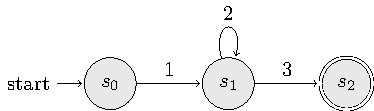
\includegraphics{chapters/cpsystems/ruleset1statemachine.pdf}
    \caption[State machine diagram for the system in \cref{rules:cps:slowmulti}]{State machine diagram for the system in \cref{rules:cps:slowmulti}.  Nodes are labelled with states, and edges with rules transitioning between them}
    \label{fig:cps:slowmulti}
\end{figure}

In particular, it is not possible here to make the second rule work in parallel --- a given functor or atom may only be used in one rule application per system step, and so the first rule application would take exclusive control of both the \(c\) functor and its \(d\) contents, preventing any further rule applications from occurring.  A further wrinkle of this \gls{ruleset} is the fact that it requires an extra temporary functor, \(f\), to store copies of the \(d\) atoms for transfer back into \(c\) at the end because the appropriate termination point for these rules can only be detected when \(c\) has been emptied.

\subsection{A Solution}
To avoid this problem, we revisit and clarify an older and rarely used operation that permits a rule to be applied to the contents of a sub-cell or functor, \emph{without} also seizing control (i.e. locking) of the sub-cell or functor itself.  We term this operation \emph{\gls{ms}}, representing the idea that as-minimal-as-possible modification is made to the containing object while modifying its contents.  We denote \glspl{ms} through the use of curly braces, rather than the usual parentheses for complex terms.  They are still complex terms, but the operation performed on them differs.  Due to this differing operation, every instance of a \gls{ms} on the \gls{lhs} \emph{must} have a matching instance on the \gls{rhs}.

% \cpruleinline{
% \cprule*{s_0}{}{\cponce}{s_1}{\cpfunc{e}{\cpempty}}
% \cprule*{s_1}{\cpfuncms{e}{\cpempty}}{\cpmaxpar}{s_2}{\cpfuncms{e}{B}~|~\cpfunc{c}{d\cpdiscard}~|~\cpfunc{a}{B}}}

% \begin{cprulesetfloat}
%     \begin{cpruleset}
%         \cprule{s_0}{}{\cponce}{s_1}{\cpfunc{e}{\cpempty}}

%         \cprule{s_1}{\cpfuncms{e}{\cpempty}}{\cpmaxpar}{s_2}{\cpfuncms{e}{B}}
%         \cppromoter{\cpfunc{c}{d\cpdiscard}}
%         \cppromoter{\cpfunc{a}{B}}
%     \end{cpruleset}
%     \caption{\label{rules:cps:microsurg}Rules for a destructive multiplication process that requires exactly two steps regardless of the numbers multiplied by using \gls{cps} \glspl{ms}}
% \end{cprulesetfloat}

\begin{cprulesetfloat}
    \begin{cpruleset}
        \cprule{s_0}{}{\cponce}{s_1}{\cpfunc{e}{\cpempty}}

        \cprule{s_1}{\cpfuncms{e}{\,}}{\cpmaxpar}{s_2}{\cpfuncms{e}{B}}
        \cppromoter{\cpfunc{c}{d\cpdiscard}}
        \cppromoter{\cpfunc{a}{B}}
    \end{cpruleset}
    \caption{\label{rules:cps:microsurg}Rules for a destructive multiplication process that requires exactly two steps regardless of the numbers multiplied by using \gls{cps} \glspl{ms}}
\end{cprulesetfloat}

\Cref{rules:cps:microsurg} is an example of three rules using \glspl{ms} that achieve in \emph{two} steps the same destructive multiplication as the \gls{ruleset} listed in \cref{rules:cps:slowmulti}, which requires \(D + 1\) steps.  Crucially, the second rule is still \emph{one} rule application, but the insertion of \(B\) into \(e\) happens once for each possible match on the promoter.  The use of \(c(d\cpdiscard)\) combined with the maximally parallel rule mode means that the rule will take control of and execute once for each \(d\) atom in the multiset labelled by the \(c\) functor.  As such, three lots of \(B\) will be inserted into \(e\) simultaneously while executing this rule under the example described above.

% Furthermore, non-destructive division of \(d\) by \(e\), \(d \div e = f\), could be:
% \cpruleinline{\cprule*{s_1}{\cpfuncms{f}{\cpempty}~\cpfuncms{d}{E}}{\cpmaxpar}{s_1}{f[\cpundig]~\cpfuncms{d}{\cpempty}~|~\cpfunc{e}{E}}}

% Furthermore, destructive division of \(d\) by \(e\), \(d \div e = f\), could be:
% \cpruleinline{\cprule*{s_1}{\cpfuncms{f}{\cpempty}~\cpfuncms{d}{E}}{\cpmaxpar}{s_1}{\cpfuncms{f}{\cpundig}~\cpfuncms{d}{\cpempty}~|~\cpfunc{e}{E}}}

Furthermore, destructive division of \(d\) by \(e\), \(d \div e = f\), could be:
\cpruleinline{\cprule*{s_1}{\cpfuncms{f}{\,}~\cpfuncms{d}{E}}{\cpmaxpar}{s_1}{\cpfuncms{f}{\cpundig}~\cpfuncms{d}{\,}~|~\cpfunc{e}{E}}}

Note that in the case of division, the quotient returned in the \(f\) term will be the \emph{floor} of the precise division result, i.e. the equation could be written as \(\lfloor d \div e \rfloor = f\).  For cases where the dividend is an exact multiple of the divisor, this will be the same as the correct result.  Otherwise, it will be the correct result's whole-number part only.  E.g. referring to the rule immediately above, for \(d(6)~\&~e(3)\), the output will be \(f(2)\), whereas for \(d(5)~\&~e(3)\), the output will be \(f(1)\), with the two left-over unary digits remaining in \(d\).  In other words, \(f\) receives the quotient, and \(d\) keeps the remainder.

\lstset{xleftmargin=.5in, xrightmargin=.5in} 
\begin{lstlisting}
  $\cpfuncms{a}{\cpundig} \; \rightarrow_{\cpmaxpar} \; \cpfuncms{a}{B}~|~\cpfunc{b}{B}$ #\hfill\textsl{single-step multiplication}\enspace#
  $\cpfuncms{a}{C} \; \cpfuncms{b}{\,} \; \rightarrow_{\cpmaxpar} \; \cpfuncms{a}{\,} \; \cpfuncms{b}{\cpundig}~|~\cpfunc{c}{C}$ #\hfill\textsl{single-step floor division}\enspace#
\end{lstlisting}

% To instead achieve ceiling division, first copy the dividend into the receiving term (in the example above, this would be the \(f\) term), and then withdrawing multiples of the divisor from there.  An integer multiple of the divisor will be withdrawn from the receiving term, and the copies of the unary digit added back form the quotient of the division.  The remainder of the division will also be in the receiving term, as it is not removed during the step.  Continuing with the example above, if the contents of the \(d\) term have already been copied into the \(f\) term, then ceiling division can be perfomed via:
\cpruleinline{\cprule*{s_1}{\cpfuncms{f}{E}}{\cpmaxpar}{s_1}{\cpfuncms{f}{\cpundig}~|~\cpfunc{e}{E}}}
%-----------------------------------------------------------------------------------
\section{\label{sec:cps:compoundterms}Indexed notation for compound terms}
%-----------------------------------------------------------------------------------

\emph{Indexed compound terms} are reasonably common in \gls{cps}.  That is, terms tagged with one or more sub-terms used to distinguish different instances of the same functor type.  They are still classic \gls{cps} objects with nested terms, but some of the subterms are used only to distinguish between instances of the encompassing compound term.  This is roughly analogous to tagging a term with its index in a logical vector/array or its key in a typical \fxerror{Need to distinguish this from, or integrate it with, the discussion about data structures above.}{dictionary/associative array data structure.}

For example, in \cref{chap:nmp}, compound \(v\) terms appear in multiple rules.  Ordinarily, these would be represented as nested terms along the lines of
\[ \cpfunc{v}{\cpfunc{v'}{N} \; \cpfunc{v''}{G}\; D} \]
These are used inside \glspl{tlc} to represent sets of tagged data.  They are indexed by neighbour \(N\) and tagged with a `generation count' \(G\) (further explained in \cref{sec:nmp:pespecific}).  Both of these values track metadata about a datum.  Lastly, the datum stored by the encompassing term is given.  In many common programming languages, accessing each datum might be written like \texttt{v[N]}, where \texttt{v} is a dictionary indexed by neighbour.  The \(v\) functors could be written as \[ \cpvv{N}{G}{D} \] for a shorthand that can be expanded back out to a complete form automatically.  The first pair of parentheses selects functors by neighbour, the second records the generation, while the final pair shows the actual contents.  This is \emph{purely} a notational convenience, without impact upon the application of the rules and evolution of the system.  When a concrete instance of a \(v\) compound term is indexed by a ground term (i.e. not a variable) \(k\), e.g. \(\cpvv{k}{\_}{\_}\), it may be referred to as \emph{k-tagged}.

\lstset{xleftmargin=.5in, xrightmargin=.5in} 
\begin{lstlisting}
  $\cpfunc{v}{\cpfunc{v'}{N} \; \cpfunc{v''}{G}\; D}$ #\hfill\textsl{nested functor}\enspace#
  $\cpvv{N}{G}{D}$ #\hfill\textsl{compound term}\enspace#
\end{lstlisting}
% %-----------------------------------------------------------------------------------
% \section{\label{sec-min}Efficient minimum-finding with cP~rules}
% %-----------------------------------------------------------------------------------

% Consider an unstructured multiset $A \subseteq \mathbb{N}$ of size \(n\). 
% It is well known that (1) any sequential algorithm that finds its minimum needs at least \(n\) steps, and 
% (2) any parallel algorithm that finds its minimum needs at least \(\log n\) parallel steps.

% Without loss of generality, consider a \gls{cps} cell, in state \(s_1\), where multiset \(A\) is given via functor \(a\); 
% e.g., multiset \(A = \{ 1, 2, 2, 5 \}\) is represented as \(\cpfunc{a}{1} \, \cpfunc{a}{2} \, \cpfunc{a}{2} \, \cpfunc{a}{5}\).
% The following \glspl{ruleset} implement various versions of a \gls{cps} minimum-finding algorithm.
% All these \glspl{ruleset} transit to state \(s_2\) and construct a term with functor \(b\), containing \(\mathop{min} A\).
% Some of these are destructive processes; if otherwise desired, one could first make a copy of the initial multiset \(A\).

% The following destructive \gls{ruleset} emulates the classical sequential minimum finding algorithm, which takes \(n\) steps:

% \lstset{xleftmargin=.5in, xrightmargin=.5in} 
% \begin{lstlisting}
% $s_1$  $\cpfunc{a}{X}$  $\rightarrow_{1}$  $s_2$  $\cpfunc{b}{X}$ 
% $s_2$  $\cpfunc{a}{XY}$  $\cpfunc{b}{X}$  $\rightarrow_{\cponce}$  $s_2$  $\cpfunc{b}{X}$     #\hfill  $a \geq b  $ \enspace #
% $s_2$  $\cpfunc{a}{X}$  $\cpfunc{b}{X1Y}$  $\rightarrow_{\cponce}$  $s_2$  $\cpfunc{b}{X}$   #\hfill  $a < b  $ \enspace #
% \end{lstlisting}

% The following destructive \gls{ruleset} emulates the classical parallel minimum finding algorithm, which takes \(\log n\) steps.
% As long as there is more than one term \(a\), the \gls{ruleset} loops in state \(s_1\), keeping minima between pairs.
% When only one \(a\) remains (containing the minimum value), the \gls{ruleset} transits to state \(s_2\) and tags the minimum. 

% \lstset{xleftmargin=.5in, xrightmargin=.5in} 
% \begin{lstlisting}
% $s_1$  $\cpfunc{a}{XY}$  $\cpfunc{a}{X}$  $\rightarrow_{\cpmaxpar}$  $s_1$  $\cpfunc{a}{X}$     
% $s_1$  $\cpfunc{a}{X}$  $\cpfunc{a}{X1Y}$  $\rightarrow_{\cpmaxpar}$  $s_1$  $\cpfunc{a}{X}$
% $s_1$  $\cpfunc{a}{X}$  $\rightarrow_{\cponce}$  $s_2$  $\cpfunc{b}{X}$  
% \end{lstlisting}

% However, using the full associative power of \gls{cps}, we can find a non-destructive version with two rules, 
% which works in \emph{just two steps} (regardless of the set cardinality). 
% This is a substantial improvement over existing classical algorithms (both sequential and parallel). 
% It starts by making a full copy of \(a\) as \(b\), in one \(\cpmaxpar\)-parallel step, 
% and then deletes all non-minimal \(b\) values in another \(\cpmaxpar\)-parallel step. 

% \lstset{xleftmargin=.5in, xrightmargin=.5in} 
% \begin{lstlisting}
% $s_1$  $\rightarrow_{\cpmaxpar}$  $s_1'$  $\cpfunc{b}{X}$    $\mid$  $\cpfunc{a}{X}$  
% $s_1'$  $\cpfunc{b}{X1Y}$  $\rightarrow_{\cpmaxpar}$  $s_2$    $\mid$  $\cpfunc{a}{X}$  
% \end{lstlisting}

% Note that if the minimum value appears several times in multiset \(A\), 
% then we will end with the same multiplicity of \(b\)'s, each one containing the same value, \(\mathop{min} A\).
% If required, there are several ways to select only one copy and delete the rest, but we do not deal with this issue further here.

% Moreover, using the full power of cP~inhibitors (as logical negations, with local variables), 
% we can even non-destructively solve the problem in just \emph{one single step},
% with one or two rules.
% This version is implemented by the following \gls{ruleset}:

% \lstset{xleftmargin=.5in, xrightmargin=.5in} 
% \begin{lstlisting}
% $s_1$  $\rightarrow_{\cponce}$  $s_2$  $\cpfunc{b}{}$    $\mid$  $\cpfunc{a}{}$
% $s_1$  $\rightarrow_{\cponce}$  $s_2$  $\cpfunc{b}{1Z}$     $\mid$  $\cpfunc{a}{1Z}$     $\neg$  $(Z=XY)$  $\cpfunc{a}{X}$
% \end{lstlisting}

% If \(A\) contains zero, then there is a term \(\cpfunc{a}{}\), and: (1) the first rule applies, constructing \(\cpfunc{b}{}\); (2) the second rule is not applicable.
% Otherwise, (if there is no zero in \(A\)): (1) the first rule is not applicable; (2) the second rule constructs \(\cpfunc{b}{1Z}\), 
% a value which exists among \(a\)'s, as \(\cpfunc{a}{1Z}\), but there is NO other \(a\) containing a strictly lesser value, such as \(\cpfunc{a}{X}\),
% where \(X\) is a sub-multiset of \(Z\), \(X \subseteq Z\).
% Finally, the newly constructed \(b\) will contain one copy of the minimum value of multiset \(A\).

% If multiset \(A\) does not contain zero values, i.e. \(A \subseteq \mathbb{N}^+\), then the first rule can be safely omitted (as it will never be applicable). 
% A similar \gls{ruleset} can be devised for finding the maximum of a given set of natural numbers.

% %%%%%%%%%%%%%%%%%%%%%%%%%%%%%%%%%%%%%%%%%%%%%%%%%%%%%%%%%%%%%%%%%%%%%%%%%%%%%%%%%%%%%%%%
% %%%%%%%%%%%%%%%%%%%%%%%%%%%%%%%%%%%%%%%%%%%%%%%%%%%%%%%%%%%%%%%%%%%%%%%%%%%%%%%%%%%%%%%%
% %%%%%%%%%%%%%%%%%%%%%%%%%%%%%%%%%%%%%%%%%%%%%%%%%%%%%%%%%%%%%%%%%%%%%%%%%%%%%%%%%%%%%%%%
% %%%%%%%%%%%%%%%%%%%%%%%%%%%%%%%%%%%%%%%%%%%%%%%%%%%%%%%%%%%%%%%%%%%%%%%%%%%%%%%%%%%%%%%%

%-----------------------------------------------------------------------------------
\section{Statistical Operations}\label{sec:cps:stats}
%-----------------------------------------------------------------------------------

This section presents and discusses procedures in \gls{cps} for the following fundamental statistical operations on numerical sets and multisets:
\begin{itemize}
    \item Finding the minimum and maximum elements.
    \item Determining the overall number and counting the frequency of elements.
    \item Computing the sum, mean, and mode over all elements.
    \item Sorting elements.
    \item Selecting the \(n^{\text{th}}\) (and thus median) element.
\end{itemize}

Leveraging the power of \gls{cps} -- logical pattern matching on associative data objects -- \emph{all} of the presented procedures run in constant time O\((1)\) and require small, fixed \glspl{ruleset} for all cases.  For brevity, these rules consider only the case of non-empty (multi)sets of natural numbers greater than zero (\(\mathbb{N}^+\)), and their total order (\(\leq\)).  Extensions to handle zero values and empty sets are not complicated, but would inflate \glspl{ruleset} by a few additional rules without adding significant value (although they would not alter the time complexity).

At the start (``step 0'') of each presented operation, assume an arbitrary non-empty set or multiset of \(s\) objects, which each hold an arbitrary number.  For each example with a set, the starting \(s\) terms assumed present are:  \[S_1 = \cpset{\cpfunc{s}{2}, \cpfunc{s}{3}, \cpfunc{s}{5}, \cpfunc{s}{6}, \cpfunc{s}{7}}\]  Likewise, the assumed multiset is \[S_2 = \cpset{\cpfunc{s}{2}, \cpfunc{s}{2}, \cpfunc{s}{3}, \cpfunc{s}{5}, \cpfunc{s}{5}, \cpfunc{s}{6}, \cpfunc{s}{6}, \cpfunc{s}{6}, \cpfunc{s}{7}}\]  In almost all cases, the operations apply equally to sets and multisets, so the examples assume the presence of \(S_2\) inside the top-level cell.  The exceptions to that are in \cref{sec:cps:sortsets} and \cref{sec:cps:selectsets}, where \(S_1\) is assumed instead, and \cref{sec:cps:sortmultisetid} and \cref{sec:cps:sortmultisetid}, which use \(S_2\) with an additional datum for each element.  The rules provided are all non-destructive with respect to the (multi)set \(S\).  Destructive versions are simple to derive from the non-destructive ones, so are omitted.

In all cases, the rules are written so that the final result is found in one or more \(r\) functor objects, as appropriate.  Examples of the evolution are given in tabular form immediately after the rules for each operation.  Each table lists \emph{only} the newly created, modified, and deleted objects in the top-level cell at the end of that step.  Modified objects are presented with their outermost functor in boldface, e.g., \(\cpfunc{r}{0}\) to \(\mathbf{\cpfunc{r}{4}}\).  Deleted objects are struck out, e.g., \(\cpfunc{r'}{2}\) to \sout{\(\cpfunc{r'}{2}\)}.

%%%%%%%%%%%%%%%%%%

%-------------------------------------------------------
\subsection{\label{sec:cps:minmax}Minimum and Maximum}
%-------------------------------------------------------

%-----------------------------------------------------------------------------------
% \section{\label{sec-min}Efficient minimum-finding with cP~rules}
%-----------------------------------------------------------------------------------

Consider an unstructured multiset $A \subseteq \mathbb{N}$ of size \(n\). 
It is well known that (1) any sequential algorithm that finds its minimum needs at least \(n\) steps, and 
(2) any parallel algorithm that finds its minimum needs at least \(\log n\) parallel steps.

Without loss of generality, consider a \gls{cps} cell, in state \(s_1\), where multiset \(A\) is given via functor \(a\); 
e.g., multiset \(A = \{ 1, 2, 2, 5 \}\) is represented as \(\cpfunc{a}{1} \, \cpfunc{a}{2} \, \cpfunc{a}{2} \, \cpfunc{a}{5}\).
The following \glspl{ruleset} implement various versions of a \gls{cps} minimum-finding algorithm.
All these \glspl{ruleset} transit to state \(s_2\) and construct a term with functor \(b\), containing \(\mathop{min} A\).
Some of these are destructive processes; if otherwise desired, one could first make a copy of the initial multiset \(A\).

The following destructive \gls{ruleset} emulates the classical sequential minimum finding algorithm, which takes \(n\) steps:

\lstset{xleftmargin=.5in, xrightmargin=.5in} 
\begin{lstlisting}
$s_1$  $\cpfunc{a}{X}$  $\rightarrow_{1}$  $s_2$  $\cpfunc{b}{X}$ 
$s_2$  $\cpfunc{a}{XY}$  $\cpfunc{b}{X}$  $\rightarrow_{\cponce}$  $s_2$  $\cpfunc{b}{X}$     #\hfill  $a \geq b  $ \enspace #
$s_2$  $\cpfunc{a}{X}$  $\cpfunc{b}{X1Y}$  $\rightarrow_{\cponce}$  $s_2$  $\cpfunc{b}{X}$   #\hfill  $a < b  $ \enspace #
\end{lstlisting}

The following destructive \gls{ruleset} emulates the classical parallel minimum finding algorithm, which takes \(\log n\) steps.
As long as there is more than one term \(a\), the \gls{ruleset} loops in state \(s_1\), keeping minima between pairs.
When only one \(a\) remains (containing the minimum value), the \gls{ruleset} transits to state \(s_2\) and tags the minimum. 

\lstset{xleftmargin=.5in, xrightmargin=.5in} 
\begin{lstlisting}
$s_1$  $\cpfunc{a}{XY}$  $\cpfunc{a}{X}$  $\rightarrow_{\cpmaxpar}$  $s_1$  $\cpfunc{a}{X}$     
$s_1$  $\cpfunc{a}{X}$  $\cpfunc{a}{X1Y}$  $\rightarrow_{\cpmaxpar}$  $s_1$  $\cpfunc{a}{X}$
$s_1$  $\cpfunc{a}{X}$  $\rightarrow_{\cponce}$  $s_2$  $\cpfunc{b}{X}$  
\end{lstlisting}

However, using the full associative power of \gls{cps}, we can find a non-destructive version with two rules, 
which works in \emph{just two steps} (regardless of the set cardinality). 
This is a substantial improvement over existing classical algorithms (both sequential and parallel). 
It starts by making a full copy of \(a\) as \(b\), in one \(\cpmaxpar\)-parallel step, 
and then deletes all non-minimal \(b\) values in another \(\cpmaxpar\)-parallel step. 

\lstset{xleftmargin=.5in, xrightmargin=.5in} 
\begin{lstlisting}
$s_1$  $\rightarrow_{\cpmaxpar}$  $s_1'$  $\cpfunc{b}{X}$    $\mid$  $\cpfunc{a}{X}$  
$s_1'$  $\cpfunc{b}{X1Y}$  $\rightarrow_{\cpmaxpar}$  $s_2$    $\mid$  $\cpfunc{a}{X}$  
\end{lstlisting}

Note that if the minimum value appears several times in multiset \(A\), 
then we will end with the same multiplicity of \(b\)'s, each one containing the same value, \(\mathop{min} A\).
If required, there are several ways to select only one copy and delete the rest, but we do not deal with this issue further here.

Moreover, using the full power of cP~inhibitors (as logical negations, with local variables), 
we can even non-destructively solve the problem in just \emph{one single step},
with one or two rules.
This version is implemented by the following \gls{ruleset}:

\lstset{xleftmargin=.5in, xrightmargin=.5in} 
\begin{lstlisting}
$s_1$  $\rightarrow_{\cponce}$  $s_2$  $\cpfunc{b}{}$    $\mid$  $\cpfunc{a}{}$
$s_1$  $\rightarrow_{\cponce}$  $s_2$  $\cpfunc{b}{1Z}$     $\mid$  $\cpfunc{a}{1Z}$     $\neg$  $(Z=XY)$  $\cpfunc{a}{X}$
\end{lstlisting}

If \(A\) contains zero, then there is a term \(\cpfunc{a}{}\), and: (1) the first rule applies, constructing \(\cpfunc{b}{}\); (2) the second rule is not applicable.
Otherwise, (if there is no zero in \(A\)): (1) the first rule is not applicable; (2) the second rule constructs \(\cpfunc{b}{1Z}\), 
a value which exists among \(a\)'s, as \(\cpfunc{a}{1Z}\), but there is NO other \(a\) containing a strictly lesser value, such as \(\cpfunc{a}{X}\),
where \(X\) is a sub-multiset of \(Z\), \(X \subseteq Z\).
Finally, the newly constructed \(b\) will contain one copy of the minimum value of multiset \(A\).

If multiset \(A\) does not contain zero values, i.e. \(A \subseteq \mathbb{N}^+\), then the first rule can be safely omitted (as it will never be applicable). 
A similar \gls{ruleset} can be devised for finding the maximum of a given set of natural numbers.

The rules of this \namecref{sec:cps:minmax} apply equally to sets and multisets.  The \glspl{ruleset} of this  \namecref{sec:cps:minmax} are notable as being two of only three in this work to use inhibitors, while the third, \cref{rules:cps:mode}, essentially performs maximum selection as part of its process.  An alternative approach forgoing inhibitors is described in \cite{Nicolescu2018} if needed.

%-----------------------------------------
\subsubsection{Minimum --- O\((1)\)}\label{sec:cps:min}
%-----------------------------------------

\begin{proposition}\label{prop:cps:min}
Finding the minimum takes one step.
\end{proposition}

\begin{proof}
Consider \cref{rules:cps:min} and the example in \cref{tab:cps:min}.  The rule to find the minimum selects an \(s\) term's value, such that there is no other \(s\) with a strictly lower value.
\end{proof}

\begin{cprulesetfloat}
\begin{cpruleset}
\cprule*{s_1}{}{\cponce}{s_2}{\cpfunc{r}{R\cpundig T}}
\cppromoter{\cpfunc{s}{R\cpundig T}}
\cpinhibitor{\cpfunc{s}{R}}
\end{cpruleset}
\caption{\label{rules:cps:min}\Gls{ruleset} to find the minimum element in a (multi)set}
\end{cprulesetfloat}

\begin{table}
\centering
\begin{tabular}{|r|l|}
    \hline
    \textbf{Step} & \textbf{New, Modified or Deleted Objects} \\ \hline
    1 & \(\cpfunc{r}{2}\)\\ \hline
\end{tabular}
\caption[Example evolution of \cref{rules:cps:min}]{\label{tab:cps:min}Example evolution of \cref{rules:cps:min} starting on multiset \(S_2\)}
\end{table}

%-----------------------------------------
\subsubsection{\label{sec:cps:max}Maximum --- O\((1)\)}
%-----------------------------------------

\begin{proposition}\label{prop:cps:max}
Finding the maximum takes one step.
\end{proposition}

\begin{proof}
Consider \cref{rules:cps:max} and the example in \cref{tab:cps:max}.  The rule to find the maximum selects an \(s\) term's value, such that there is no other \(s\) with a strictly higher value.
\end{proof}

\begin{cprulesetfloat}
\begin{cpruleset}

\cprule*{s_1}{}{\cponce}{s_2}{\cpfunc{r}{R}}
\cppromoter{\cpfunc{s}{R}}
\cpinhibitor{\cpfunc{s}{R\cpundig \_}}

\end{cpruleset}
\caption{\label{rules:cps:max}\Gls{ruleset} to find the maximum element in a (multi)set}
\end{cprulesetfloat}

\begin{table} \centering
\begin{tabular}{|r|l|}
    \hline
    \textbf{Step} & \textbf{New, Modified or Deleted Objects} \\ \hline
    1 & \(\cpfunc{r}{7}\)\\ \hline
\end{tabular} 
\caption[Example evolution of \cref{rules:cps:max}]{\label{tab:cps:max}Example evolution of \cref{rules:cps:max} starting on multiset \(S_2\)}
\end{table}

%%%%%%%%%%%%%%%%%%

%-------------------------------------------------------
\subsection{Counting}\label{sec:cps:counting}
%-------------------------------------------------------

%-----------------------------------------
\subsubsection{Counting Elements --- O\((1)\)}\label{sec:cps:countelems}
%-----------------------------------------

\begin{proposition}\label{prop:cps:countelems}
Determining the magnitude of a (multi)set takes two steps.
\end{proposition}

\begin{proof}
Consider \cref{rules:cps:countelems} and the example in \cref{tab:cps:countelems}.  The first rule creates an empty term to store the result, and then the second rule tallies the elements present.
\end{proof}

\begin{cprulesetfloat} \begin{cpruleset}

\cprule{s_1}{}{\cponce}{s_2}{\cpfunc{r}{\cpempty}}

\cprule{s_2}{\cpfuncms{r}{\,}}{\cpmaxpar}{s_3}{\cpfuncms{r}{\cpundig}}
\cppromoter{\cpfunc{s}{\_}}

\end{cpruleset}
\caption{\label{rules:cps:countelems}\Gls{ruleset} to find the magnitude of a (multi)set}
\end{cprulesetfloat}

\begin{table} \centering
   \begin{tabular}{|r|l|}
    \hline
    \textbf{Step} & \textbf{New, Modified or Deleted Objects} \\ \hline
    1 & \(\cpfunc{r}{0}\)\\ \hline
    
    2 & \(\mathbf{\cpfunc{r}{9}}\)\\ \hline
\end{tabular}
\caption[Example evolution of \cref{rules:cps:countelems}]{\label{tab:cps:countelems}Example evolution of \cref{rules:cps:countelems} starting on multiset \(S_2\)}
\end{table}

%-----------------------------------------
\subsubsection{Counting Frequency of Elements --- O\((1)\)}\label{sec:cps:countfreq}
%-----------------------------------------

\begin{proposition}\label{prop:cps:countfreq}
Counting the occurrence -- essentially creating a histogram -- of the values in a multiset takes three steps.
\end{proposition}

\begin{proof}
Consider \cref{rules:cps:countfreq} and the example in \cref{tab:cps:countfreq}.  The first rule creates a tally \(r\) term for every \(s\) term, while the second rule eliminates any ensuing duplicates, leaving only one \(r\) per unique value stored in any \(s\).  Lastly, rule 3 performs a similar operation to \cref{sec:cps:countelems}, incrementing each \(r\) term's tally by one for each \(s\) term containing the corresponding value.
\end{proof}

% \cpresetrulenumber
\begin{cprulesetfloat}
\begin{cpruleset}
\cprule{s_1}{}{\cpmaxpar}{s_2}{\cpfuncn{r}{R}{\cpempty}}
\cppromoter{\cpfunc{s}{R}}

\cprule{s_2}{\cpfuncn{r}{R}{\_}}{\cpmaxpar}{s_3}{}
\cppromoter{\cpfuncn{r}{R}{\_}}

\cprule{s_3}{\cpfuncnms{r}{R}{\,}}{\cpmaxpar}{s_4}{\cpfuncnms{r}{R}{\cpundig}}
\cppromoter{\cpfunc{s}{R}}
\end{cpruleset}
\caption{\label{rules:cps:countfreq}\Gls{ruleset} to count the occurrence frequency of elements in a multiset}
\end{cprulesetfloat}

\begin{table} \centering
   \begin{tabular}{|r|l|}
    \hline
    \textbf{Step} & \textbf{New, Modified or Deleted Objects} \\ \hline
    1 & \(\cpfuncn{r}{2}{0}\), \(\cpfuncn{r}{2}{0}\), \(\cpfuncn{r}{3}{0}\), \(\cpfuncn{r}{5}{0}\), \(\cpfuncn{r}{5}{0}\), \(\cpfuncn{r}{6}{0}\), \(\cpfuncn{r}{6}{0}\), \(\cpfuncn{r}{6}{0}\), \(\cpfuncn{r}{7}{0}\)\\ \hline
    
    % 2 & \sout{\(\cpfuncn{r}{2}{0}\)}, \sout{\(\cpfuncn{r}{5}{0}\)}, \sout{\(\cpfuncn{r}{6}{0}\)}, \sout{\(\cpfuncn{r}{6}{0}\)}\\ \hline
    
    2 & \(\cpfuncn{r}{2}{0}\), \sout{\(\cpfuncn{r}{2}{0}\)}, \(\cpfuncn{r}{3}{0}\), \(\cpfuncn{r}{5}{0}\), \sout{\(\cpfuncn{r}{5}{0}\)}, \(\cpfuncn{r}{6}{0}\), \sout{\(\cpfuncn{r}{6}{0}\)}, \sout{\(\cpfuncn{r}{6}{0}\)}, \(\cpfuncn{r}{7}{0}\)\\ \hline
    
    3 & \(\mathbf{\cpfuncn{r}{2}{2}}\), \(\mathbf{\cpfuncn{r}{3}{1}}\), \(\mathbf{\cpfuncn{r}{5}{2}}\), \(\mathbf{\cpfuncn{r}{6}{3}}\), \(\mathbf{\cpfuncn{r}{7}{1}}\)\\ \hline
\end{tabular}
\caption[Example evolution of \cref{rules:cps:countfreq}]{\label{tab:cps:countfreq}Example evolution of \cref{rules:cps:countfreq} starting on multiset \(S_2\)}
\end{table}

\Cref{rules:cps:countfreq} works equally well for sets, but the frequency of each element present will be one due to the nature of a set.

%-------------------------------------------------------
\subsection{Sum, Mean and Mode}\label{sec:cps:sumeanmode}
%-------------------------------------------------------

%-----------------------------------------
\subsubsection{Sum --- O\((1)\)}\label{sec:cps:sum}
%-----------------------------------------

\begin{proposition}\label{prop:cps:sum}
Computing the sum of the elements in a (multi)set requires two steps.
\end{proposition}

\begin{proof}
Consider \cref{rules:cps:sum} and the example in \cref{tab:cps:sum}.  These rules act very similarly to \cref{sec:cps:countelems}, but add the total stored value in every \(s\) term to the \(r\) term, rather than simply one \(\cpundig\) per \(s\) term.
\end{proof}

% \cpresetrulenumber
\begin{cprulesetfloat} \begin{cpruleset}
\cprule{s_1}{}{\cponce}{s_2}{\cpfunc{r}{\cpempty}}
\cprule{s_2}{\cpfuncms{r}{\,}}{\cpmaxpar}{s_3}{\cpfuncms{r}{R}}
\cppromoter{\cpfunc{s}{R}}
\end{cpruleset}
\caption{\label{rules:cps:sum}\Gls{ruleset} to find the sum of numeric elements in a (multi)set}
\end{cprulesetfloat}

\begin{table} \centering
   \begin{tabular}{|r|l|}
    \hline
    \textbf{Step} & \textbf{New, Modified or Deleted Objects} \\ \hline
    1 & \(\cpfunc{r}{0}\)\\ \hline
    2 & \(\cpfunc{r}{42}\)\\ \hline

\end{tabular}
\caption[Example evolution of \cref{rules:cps:sum}]{\label{tab:cps:sum}Example evolution of \cref{rules:cps:sum} starting on multiset \(S_2\)}
\end{table}

%-----------------------------------------
\subsubsection{Mean --- O\((1)\)}\label{sec:cps:mean}
%-----------------------------------------

\begin{proposition}\label{prop:cps:mean}
Finding the (whole number) mean of a (multi)set requires four steps.
\end{proposition}

\begin{proof}
Consider \cref{rules:cps:mean} and the example in \cref{tab:cps:mean}.  Computing the mean is mostly a combination of two previous operations:  Sum the elements (\cref{sec:cps:sum}), and divide by the count of elements (\cref{sec:cps:countelems}).  The summing and counting may be performed simultaneously in two steps, with two extra steps for the division.
\end{proof}

% \cpresetrulenumber
\begin{cprulesetfloat}
\begin{cpruleset}
\cprule{s_1}{}{\cponce}{s_2}{\cpfunc{c}{\cpempty} \; \cpfunc{r}{\cpempty} \; \cpfunc{r'}{\cpempty}}

\cprule{s_2}{\cpfuncms{c}{\,}}{\cpmaxpar}{s_3}{\cpfuncms{c}{\cpundig}}
\cppromoter{\cpfunc{s}{\_}}

\cprule{s_2}{\cpfuncms{r}{\,} \; \cpfuncms{r'}{\,}}{\cpmaxpar}{s_3}{\cpfuncms{r}{R} \; \cpfuncms{r'}{R}}
\cppromoter{\cpfunc{s}{R}}

\cprule{s_3}{\cpfuncms{r}{C} \; \cpfuncms{r'}{C}}{\cpmaxpar}{s_4}{\cpfuncms{r}{\cpundig} \; \cpfuncms{r'}{\,}}
\cppromoter{\cpfunc{c}{C}}

\cprule{s_4}{\cpfunc{r}{QR} \; \cpfunc{r'}{R}}{\cponce}{s_5}{\cpfunc{r}{Q}}
\end{cpruleset}
\caption{\label{rules:cps:mean}\Gls{ruleset} to find the mean of elements in a (multi)set}
\end{cprulesetfloat}

\begin{table} \centering
  \begin{tabular}{|r|l|}
    \hline
    \textbf{Step} & \textbf{New, Modified or Deleted Objects} \\ \hline
    1 & \(\cpfunc{c}{0}\), \(\cpfunc{r}{0}\), \(\cpfunc{r'}{0}\)\\ \hline
    2 & \(\mathbf{\cpfunc{c}{9}}\), \(\mathbf{\cpfunc{r}{42}}\), \(\mathbf{\cpfunc{r'}{42}}\)\\ \hline
    3 & \(\mathbf{\cpfunc{r}{11}}\), \(\mathbf{\cpfunc{r'}{6}}\)\\ \hline
    4 & \(\mathbf{\cpfunc{r}{5}}\), \sout{\(\cpfunc{r'}{6}\)}\\ \hline

\end{tabular}
\caption[Example evolution of \cref{rules:cps:mean}]{\label{tab:cps:mean}Example evolution of \cref{rules:cps:mean} starting on multiset \(S_2\)}
\end{table}

Rules 4 and 5 perform ceiling integer division.  Rule 4 removes \(C\) copies of the unary digit from \(r\) and adds one copy back to it.  This is repeated as many times as possible, given the number of digits available.  What is left in \(r\) at the end of the step is, in effect, the quotient plus the remainder.  In this example, with a count of nine and a sum of forty-two, the removal can be applied four times, for a total of thirty-six unary digits removed.  Five more are added at the end of the step, meaning a total of eleven remains.  This is not the correct result of ceiling integer division but is the correct quotient (5) plus the remainder (6).  Thus, another copy of the total is kept and divided, without the quotient added back in.  This leaves rule 5 to compute the correct final result by deducting the remainder from the combined quotient and remainder.

%-----------------------------------------
\subsubsection{Mode --- O\((1)\)}  \label{sec:cps:mode}
%-----------------------------------------

\begin{proposition}\label{prop:cps:mode}
Finding the mode of the elements in a multiset requires four steps.
\end{proposition}

\begin{proof}
Consider \cref{rules:cps:mode} and the example in \cref{tab:cps:mode}.  As with the mean, this process combines other operations:  Counting the frequency of elements (\cref{sec:cps:countfreq}) takes three steps, then selecting the maximum (\cref{sec:cps:max}) uses one extra step.  Unlike in \cref{sec:cps:mean}, the aforementioned \glspl{ruleset} cannot be used concurrently to reduce the number of steps required because the maximum-finding rule must only fire once the frequency counting process has concluded.
\end{proof}

% \cpresetrulenumber
\begin{cprulesetfloat} \begin{cpruleset}
\cprule{s_1}{}{\cpmaxpar}{s_2}{\cpfuncn{c}{C}{\cpempty}}
\cppromoter{\cpfunc{s}{C}}

\cprule{s_2}{\cpfuncn{c}{C}{\_}}{\cpmaxpar}{s_3}{}
\cppromoter{\cpfuncn{c}{C}{\_}}

\cprule{s_3}{\cpfuncnms{c}{C}{\,}}{\cpmaxpar}{s_4}{\cpfuncnms{c}{C}{\cpundig}}
\cppromoter{\cpfunc{s}{C}}

\cprule{s_4}{}{\cponce}{s_5}{\cpfunc{r}{C}}
\cppromoter{\cpfuncn{c}{C}{R}}
\cpinhibitor{\cpfuncn{c}{\_}{R\cpundig \_}}

\end{cpruleset}
\caption{\label{rules:cps:mode}\Gls{ruleset} to find the mode of the elements in a multiset}
\end{cprulesetfloat}

% \begin{table} \centering
%   \begin{tabular}{|r|l|}
%     \hline
%     \textbf{Step} & \textbf{New, Modified or Deleted Objects} \\ \hline
%     1 & \(\cpfuncn{c}{2}{0}\), \(\cpfuncn{c}{2}{0}\), \(\cpfuncn{c}{3}{0}\), \(\cpfuncn{c}{5}{0}\), \(\cpfuncn{c}{5}{0}\), \(\cpfuncn{c}{6}{0}\), \(\cpfuncn{c}{6}{0}\), \(\cpfuncn{c}{6}{0}\),\\& \(\cpfuncn{c}{7}{0}\)\\ \hline
    
%     2 & \sout{\(\cpfuncn{c}{2}{0}\)}, \sout{\(\cpfuncn{c}{5}{0}\)}, \sout{\(\cpfuncn{c}{6}{0}\)}, \sout{\(\cpfuncn{c}{6}{0}\)}\\ \hline
    
%     3 & \(\mathbf{\cpfuncn{c}{2}{2}}\), \(\mathbf{\cpfuncn{c}{3}{3}}\), \(\mathbf{\cpfuncn{c}{5}{2}}\), \(\mathbf{\cpfuncn{c}{6}{3}}\), \(\mathbf{\cpfuncn{c}{7}{1}}\)\\ \hline
    
%     4 & \(\cpfunc{r}{5}\)\\ \hline
% \end{tabular}
% \caption[Example evolution of \cref{rules:cps:mode}]{\label{tab:cps:mode}Example evolution of \cref{rules:cps:mode} starting on multiset \(S_2\)}
% \end{table}

\begin{table} \centering
   \begin{tabular}{|r|l|}
    \hline
    \textbf{Step} & \textbf{New, Modified or Deleted Objects} \\ \hline
    1 & \(\cpfuncn{c}{2}{0}\), \(\cpfuncn{c}{2}{0}\), \(\cpfuncn{c}{3}{0}\), \(\cpfuncn{c}{5}{0}\), \(\cpfuncn{c}{5}{0}\), \(\cpfuncn{c}{6}{0}\), \(\cpfuncn{c}{6}{0}\), \(\cpfuncn{c}{6}{0}\), \(\cpfuncn{c}{7}{0}\)\\ \hline
    
    2 & \(\cpfuncn{c}{2}{0}\), \sout{\(\cpfuncn{c}{2}{0}\)}, \(\cpfuncn{c}{3}{0}\), \(\cpfuncn{c}{5}{0}\), \sout{\(\cpfuncn{c}{5}{0}\)}, \(\cpfuncn{c}{6}{0}\), \sout{\(\cpfuncn{c}{6}{0}\)}, \sout{\(\cpfuncn{c}{6}{0}\)}, \(\cpfuncn{c}{7}{0}\)\\ \hline
    
    3 & \(\mathbf{\cpfuncn{c}{2}{2}}\), \(\mathbf{\cpfuncn{c}{3}{3}}\), \(\mathbf{\cpfuncn{c}{5}{2}}\), \(\mathbf{\cpfuncn{c}{6}{3}}\), \(\mathbf{\cpfuncn{c}{7}{1}}\)\\ \hline
    
    4 & \(\cpfuncn{c}{2}{2}\), \(\cpfuncn{c}{3}{3}\), \(\cpfuncn{c}{5}{2}\), \(\cpfuncn{c}{6}{3}\), \(\cpfuncn{c}{7}{1}\), \(\cpfunc{r}{5}\)\\ \hline
    
\end{tabular}
\caption[Example evolution of \cref{rules:cps:mode}]{\label{tab:cps:mode}Example evolution of \cref{rules:cps:mode} starting on multiset \(S_2\)}
\end{table}

%-------------------------------------------------------
\subsection{Sorting}\label{sec:cps:sorting}
%-------------------------------------------------------

In the current context, sorting is defined as appropriately associating each datum/element in a (multi)set with an ordered index in the range \([1,n]\), where \(n\) is equal to the magnitude (count of elements) of the (multi)set.\footnote{This can easily be switched to \([0,n)\) if desired.}  At the end of the process, the values in the (multi)set shall be sorted in typical ascending numerical order by associating indices with them.

For example, in the context of \(S_2\), this will be 
\begin{align*}
    \text{Element:}& &2 &&2 &&3 &&5 &&5 &&6 &&6 &&6 &&7\\
    \text{Index:}&   &1 &&2 &&3 &&4 &&5 &&6 &&7 &&8 &&9\\
\end{align*}

\Cref{sec:cps:sortsets} \& \cref{sec:cps:sortmultisetid} associate each element with the index individually, while \cref{sec:cps:sortmultisetrange} groups identical multiset elements into ranges spanning the correct indices.

%-----------------------------------------
\subsubsection{Sorting Sets --- O\((1)\)}  \label{sec:cps:sortsets}
%-----------------------------------------

\begin{proposition}\label{prop:cps:sortsets}
Sorting sets requires two steps.
\end{proposition}

\begin{proof}
Consider \cref{rules:cps:sortsets} and the example in \cref{tab:cps:sortsets}.  The rules for sorting a set work similarly to those for counting the frequency of elements (\cref{sec:cps:countfreq}).  Instead of counting the occurrence of a particular value, however, these rules count the occurrence of values strictly less than the current value.  In each instance, this number plus one is equal to the value's correct index in the total ordering, thus sorting the values.
\end{proof}

% \cpresetrulenumber
\begin{cprulesetfloat} \begin{cpruleset}
\cprule{s_1}{}{\cpmaxpar}{s_2}{\cpfuncn{r}{R}{\cpundig}}
\cppromoter{\cpfunc{s}{R}}

\cprule{s_2}{\cpfuncnms{r}{Y}{\,}}{\cpmaxpar}{s_3}{\cpfuncnms{r}{Y}{\cpundig}}
\cppromoter{\cpfunc{s}{X}}
\cppromoter{X \subsetneq Y}
\end{cpruleset}
\caption{\label{rules:cps:sortsets}\Gls{ruleset} to sort the elements in a set}
\end{cprulesetfloat}

\begin{table} \centering
   \begin{tabular}{|r|l|}
    \hline
    \textbf{Step} & \textbf{New, Modified or Deleted Objects} \\ \hline
    1 & \(\cpfuncn{r}{2}{1}\), \(\cpfuncn{r}{3}{1}\), \(\cpfuncn{r}{5}{1}\), \(\cpfuncn{r}{6}{1}\), \(\cpfuncn{r}{7}{1}\)\\ \hline
    2 & \(\cpfuncn{r}{2}{1}\), \(\mathbf{\cpfuncn{r}{3}{2}}\), \(\mathbf{\cpfuncn{r}{5}{3}}\), \(\mathbf{\cpfuncn{r}{6}{4}}\), \(\mathbf{\cpfuncn{r}{7}{5}}\)\\ \hline

\end{tabular}
\caption[Example evolution of \cref{rules:cps:sortsets}]{\label{tab:cps:sortsets}Example evolution of \cref{rules:cps:sortsets} starting on set \(S_1\)}
\end{table}

%-----------------------------------------
\subsubsection{Sorting Multisets into Ranges --- O\((1)\)}\label{sec:cps:sortmultisetrange}
%-----------------------------------------

\begin{proposition}\label{prop:cps:sortmultisetrange}
Sorting a multiset into ordered, indexed ranges requires four steps.
\end{proposition}

\begin{proof}
Consider \cref{rules:cps:sortmultisetrange} and the example in \cref{tab:cps:sortmultisetrange}.  In these rules, the last two numbers for each ending \(t\) object give a range of indices -- with inclusive lower bounds and exclusive upper bounds -- in which the \(s\) numbers of the multiset may be found once ordered.  It requires four steps and relies on the fact that elements of the same value in a multiset are indistinguishable, and thus can be ordered among themselves arbitrarily.

% Consider \cref{rules:cps:sortmultisetrange} and the example in \crefrange{objs:cps:sortmultisetrange:0}{objs:cps:sortmultisetrange:4}.  In these rules, the last two numbers for each ending \(t\) object give a range of indices -- with inclusive lower bounds and exclusive upper bounds -- in which the \(s\) numbers of the multiset may be found once ordered.  It requires four steps and relies on the fact that elements of the same value in a multiset are indistinguishable, and thus can be ordered among themselves arbitrarily.
\end{proof}

% \cpresetrulenumber
\begin{cprulesetfloat} \begin{cpruleset}
\cprule{s_1}{}{\cpmaxpar}{s_2}{\cpfuncnn{r}{R}{\cpundig}{\cpundig}}
\cppromoter{\cpfunc{s}{R}}

\cprule{s_2}{\cpfuncnn{r}{R}{\_}{\_}}{\cpmaxpar}{s_3}{}
\cppromoter{\cpfuncnn{r}{R}{\_}{\_}}

% \cprule{s_3}{\cpfunc{r}{R}}{\cpmaxpar}{s_4}{\cpfuncnn{r}{R}{\cpundig}{\cpundig}}

\cprule{s_3}{\cpfunc{r}{Y}\{\,\}\{\,\}}{\cpmaxpar}{s_4}{\cpfunc{r}{Y}\{\cpundig\}\{\cpundig\}}
\cppromoter{\cpfunc{s}{X}}
\cppromoter{X \subsetneq Y}

\cprule{s_4}{\cpfuncnnms{r}{R}{X}{\,}}{\cpmaxpar}{s_5}{\cpfuncnnms{r}{R}{X}{\cpundig}}
\cppromoter{\cpfunc{s}{R}}

\end{cpruleset}
\caption{\label{rules:cps:sortmultisetrange}\Gls{ruleset} to sort the elements of a multiset into indexed ranges}
\end{cprulesetfloat}

\begin{table} \centering
  \begin{tabular}{|r|l|}
    \hline
    \textbf{Step} & \textbf{New, Modified or Deleted Objects} \\ \hline
    1 & \(\cpfuncnn{r}{2}{1}{1}\), \(\cpfuncnn{r}{2}{1}{1}\), \(\cpfuncnn{r}{3}{1}{1}\), \(\cpfuncnn{r}{5}{1}{1}\), \(\cpfuncnn{r}{5}{1}{1}\), \(\cpfuncnn{r}{6}{1}{1}\),\\& \(\cpfuncnn{r}{6}{1}{1}\), \(\cpfuncnn{r}{6}{1}{1}\), \(\cpfuncnn{r}{7}{1}{1}\)\\ \hline
    
    2 & \(\cpfuncnn{r}{2}{1}{1}\), \sout{\(\cpfuncnn{r}{2}{1}{1}\)}, \(\cpfuncnn{r}{3}{1}{1}\), \(\cpfuncnn{r}{5}{1}{1}\), \sout{\(\cpfuncnn{r}{5}{1}{1}\)}, \(\cpfuncnn{r}{6}{1}{1}\),\\& \sout{\(\cpfuncnn{r}{6}{1}{1}\)}, \sout{\(\cpfuncnn{r}{6}{1}{1}\)}, \(\cpfuncnn{r}{7}{1}{1}\)\\ \hline
    
    % 2 & \sout{\(\cpfuncnn{r}{2}{1}{1}\)}, \sout{\(\cpfuncnn{r}{5}{1}{1}\)}, \sout{\(\cpfuncnn{r}{6}{1}{1}\)}, \sout{\(\cpfuncnn{r}{6}{1}{1}\)}\\ \hline
    
    3 & \(\cpfuncnn{r}{2}{1}{1}\), \(\mathbf{\cpfuncnn{r}{3}{3}{3}}\), \(\mathbf{\cpfuncnn{r}{5}{4}{4}}\), \(\mathbf{\cpfuncnn{r}{6}{6}{6}}\), \(\mathbf{\cpfuncnn{r}{7}{9}{9}}\)\\ \hline
    
    4 & \(\mathbf{\cpfuncnn{r}{2}{1}{3}}\), \(\mathbf{\cpfuncnn{r}{3}{3}{4}}\), \(\mathbf{\cpfuncnn{r}{5}{4}{6}}\), \(\mathbf{\cpfuncnn{r}{6}{6}{9}}\), \(\mathbf{\cpfuncnn{r}{7}{9}{10}}\)\\ \hline
\end{tabular} 
\caption[Example evolution of \cref{rules:cps:sortmultisetrange}]{\label{tab:cps:sortmultisetrange}Example evolution of \cref{rules:cps:sortmultisetrange} starting on multiset \(S_2\)}
\end{table}

% \begin{cpobjectsfloat}
% \begin{cpobjects}
% \cpobjectsline{\cpfunc{s}{2} \, \cpfunc{s}{2} \, \cpfunc{s}{3} \, \cpfunc{s}{5} \, \cpfunc{s}{5} \, \cpfunc{s}{6} \, \cpfunc{s}{6} \, \cpfunc{s}{6} \, \cpfunc{s}{7}}
% \end{cpobjects}
% \caption{\label{objs:cps:sortmultisetrange:0} Objects inside a \gls{tlc} initially containing set \(S_2\), after step 0 of \cref{rules:cps:sortmultisetrange}.}
% \end{cpobjectsfloat}

% \begin{cpobjectsfloat}
% \begin{cpobjects}
% \cpobjectsline{\cpfunc{s}{2} \, \cpfunc{s}{2} \, \cpfunc{s}{3} \, \cpfunc{s}{5} \, \cpfunc{s}{5} \, \cpfunc{s}{6} \, \cpfunc{s}{6} \, \cpfunc{s}{6} \, \cpfunc{s}{7} \quad \cpfuncnn{r}{2}{1}{1} \; \cpfuncnn{r}{2}{1}{1}}
% \cpobjectsline{\cpfuncnn{r}{3}{1}{1} \; \cpfuncnn{r}{5}{1}{1} \; \cpfuncnn{r}{5}{1}{1} \; \cpfuncnn{r}{6}{1}{1} \; \cpfuncnn{r}{6}{1}{1} \; \cpfuncnn{r}{6}{1}{1} \; \cpfuncnn{r}{7}{1}{1}}
% \end{cpobjects}
% \caption{\label{objs:cps:sortmultisetrange:1} Objects inside a \gls{tlc} initially containing set \(S_2\), after step 1 of \cref{rules:cps:sortmultisetrange}.}
% \end{cpobjectsfloat}

% \begin{cpobjectsfloat}
% \begin{cpobjects}
% \cpobjectsline{\cpfunc{s}{2} \, \cpfunc{s}{2} \, \cpfunc{s}{3} \, \cpfunc{s}{5} \, \cpfunc{s}{5} \, \cpfunc{s}{6} \, \cpfunc{s}{6} \, \cpfunc{s}{6} \, \cpfunc{s}{7} \quad \cpfuncnn{r}{2}{1}{1} \; \cpfuncnn{r}{3}{1}{1}}
% \cpobjectsline{\cpfuncnn{r}{5}{1}{1} \; \cpfuncnn{r}{6}{1}{1} \; \cpfuncnn{r}{7}{1}{1}}
% \end{cpobjects}
% \caption{\label{objs:cps:sortmultisetrange:2} Objects inside a \gls{tlc} initially containing set \(S_2\), after step 1 of \cref{rules:cps:sortmultisetrange}.}
% \end{cpobjectsfloat}

% \begin{cpobjectsfloat}
% \begin{cpobjects}
% \cpobjectsline{\cpfunc{s}{2} \, \cpfunc{s}{2} \, \cpfunc{s}{3} \, \cpfunc{s}{5} \, \cpfunc{s}{5} \, \cpfunc{s}{6} \, \cpfunc{s}{6} \, \cpfunc{s}{6} \, \cpfunc{s}{7} \quad \cpfuncnn{r}{2}{1}{1} \; \cpfuncnn{r}{3}{3}{3}}
% \cpobjectsline{\cpfuncnn{r}{5}{4}{4} \; \cpfuncnn{r}{6}{6}{6} \; \cpfuncnn{r}{7}{9}{9}}
% \end{cpobjects}
% \caption{\label{objs:cps:sortmultisetrange:3} Objects inside a \gls{tlc} initially containing set \(S_2\), after step 1 of \cref{rules:cps:sortmultisetrange}.}
% \end{cpobjectsfloat}

% \begin{cpobjectsfloat}
% \begin{cpobjects}
% \cpobjectsline{\cpfunc{s}{2} \, \cpfunc{s}{2} \, \cpfunc{s}{3} \, \cpfunc{s}{5} \, \cpfunc{s}{5} \, \cpfunc{s}{6} \, \cpfunc{s}{6} \, \cpfunc{s}{6} \, \cpfunc{s}{7} \quad \cpfuncnn{r}{2}{1}{3} \; \cpfuncnn{r}{3}{3}{4}}
% \cpobjectsline{\cpfuncnn{r}{5}{4}{6} \; \cpfuncnn{r}{6}{6}{9} \; \cpfuncnn{r}{7}{9}{10}}
% \end{cpobjects}
% \caption{\label{objs:cps:sortmultisetrange:4} Objects inside a \gls{tlc} initially containing set \(S_2\), after step 1 of \cref{rules:cps:sortmultisetrange}.}
% \end{cpobjectsfloat}

In this example, 2s are in the index range \([1,3)\), 3s are in \([3,4)\), 5s are in \([4,6)\), 6s are in \([6,9)\) and 7s are in \([9,10)\).  This process can also sort all sets that \cref{sec:cps:sortsets} can sort (rules 1 and 3 here are closely equivalent to those rules), but the current approach includes unnecessary extra information -- every listed range would be only one step wide, so on set \(S_1\) the final result would be \(\cpfuncnn{r}{2}{1}{1}, \cpfuncnn{r}{3}{2}{2},\dots\), i.e. 2: \([1,2)\), 3: \([2,3) \dots\) -- and requires two unnecessary extra steps.

%-----------------------------------------
\subsubsection{Sorting Multisets with Unique Identifiers --- O\((1)\)}\label{sec:cps:sortmultisetid}
%-----------------------------------------

\begin{proposition}\label{prop:cps:sortmultisetid}
Sorting a multiset, when accompanied by unique identifiers for every element, requires three steps.
\end{proposition}

\begin{proof}
Consider \cref{rules:cps:sortmultisetid} and the example in \cref{tab:cps:sortmultisetid}.  This \gls{ruleset} is an extension of the rules found in \cref{sec:cps:sortsets}.  Those rules work only for sets and fail in the presence of more than one of a given element.  In effect, the rules seek to impose a \emph{strict} total ordering and contemplate only the situation where each element in the set is strictly greater than or less than another element.  Suppose there \emph{is} some additional information on each element available, such as a unique, comparable identifier for each element in the multiset. In that case, this can be used to `break ties' between elements of equal value.  In this case, the use of one extra rule suffices to impose a strict total ordering on every element and sort the multiset consistently.  These additional identifiers, included as the first value in \(s\) objects, must themselves be comparable, however.
\end{proof}

An example of the described unique identifiers can be found in \cref{sec:medianfilter}, where additional information is available based on the origin of each element in the multiset.

It is as yet unclear how to introduce a strict total ordering, as required to sort elements into specific indices, with \gls{cps} rules when some elements are effectively indistinguishable.  The ranges approach of \cref{sec:cps:sortmultisetrange} sidesteps this issue by collapsing elements of equal value into one ordered term.


% \cpresetrulenumber
\begin{cprulesetfloat} \begin{cpruleset}
\cprule{s_1}{}{\cpmaxpar}{s_2}{\cpfuncnn{r}{I}{U}{\cpundig}}
\cppromoter{\cpfuncn{s}{I}{U}}

\cprule{s_2}{\cpfuncnnms{r}{I}{Y}{\,}}{\cpmaxpar}{s_3}{\cpfuncnnms{r}{I}{Y}{\cpundig}}
\cppromoter{\cpfuncn{s}{\_}{X}}
\cppromoter{X \subsetneq Y}

\cprule{s_3}{\cpfuncnnms{r}{J}{X}{\,}}{\cpmaxpar}{s_4}{\cpfuncnnms{r}{J}{X}{\cpundig}}
\cppromoter{\cpfuncn{s}{I}{X}}
\cppromoter{I \subsetneq J}
\end{cpruleset}
\caption{\label{rules:cps:sortmultisetid}\Gls{ruleset} to sort the elements of a multiset, when each element has an accompanying unique comparable identifier}
\end{cprulesetfloat}

\begin{table} \centering
   \begin{tabular}{|r|l|}
    \hline
    \textbf{Step} & \textbf{New, Modified or Deleted Objects} \\ \hline
    0 & \(\cpfuncn{s}{8}{2}\), \(\cpfuncn{s}{3}{2}\), \(\cpfuncn{s}{7}{3}\), \(\cpfuncn{s}{5}{5}\), \(\cpfuncn{s}{1}{5}\), \(\cpfuncn{s}{6}{6}\), \(\cpfuncn{s}{2}{6}\), \(\cpfuncn{s}{9}{6}\), \(\cpfuncn{s}{4}{7}\)\\ \hline
    
    1 & \(\cpfuncn{s}{8}{2}\), \(\cpfuncn{s}{3}{2}\), \(\cpfuncn{s}{7}{3}\), \(\cpfuncn{s}{5}{5}\), \(\cpfuncn{s}{1}{5}\), \(\cpfuncn{s}{6}{6}\), \(\cpfuncn{s}{2}{6}\), \(\cpfuncn{s}{9}{6}\), \(\cpfuncn{s}{4}{7}\),\\& \(\cpfuncnn{r}{8}{2}{1}\), \(\cpfuncnn{r}{3}{2}{1}\), \(\cpfuncnn{r}{7}{3}{1}\), \(\cpfuncnn{r}{5}{5}{1}\), \(\cpfuncnn{r}{1}{5}{1}\), \(\cpfuncnn{r}{6}{6}{1}\),\\& \(\cpfuncnn{r}{2}{6}{1}\), \(\cpfuncnn{r}{9}{6}{1}\), \(\cpfuncnn{r}{4}{7}{1}\)\\ \hline
    
    2 & \(\cpfuncn{s}{8}{2}\), \(\cpfuncn{s}{3}{2}\), \(\cpfuncn{s}{7}{3}\), \(\cpfuncn{s}{5}{5}\), \(\cpfuncn{s}{1}{5}\), \(\cpfuncn{s}{6}{6}\), \(\cpfuncn{s}{2}{6}\), \(\cpfuncn{s}{9}{6}\), \(\cpfuncn{s}{4}{7}\),\\& \(\cpfuncnn{r}{8}{2}{1}\), \(\cpfuncnn{r}{3}{2}{1}\), \(\mathbf{\cpfuncnn{r}{7}{3}{3}}\), \(\mathbf{\cpfuncnn{r}{5}{5}{4}}\), \(\mathbf{\cpfuncnn{r}{1}{5}{4}}\), \(\mathbf{\cpfuncnn{r}{6}{6}{6}}\),\\& \(\mathbf{\cpfuncnn{r}{2}{6}{6}}\), \(\mathbf{\cpfuncnn{r}{9}{6}{6}}\), \(\mathbf{\cpfuncnn{r}{4}{7}{9}}\)\\ \hline
    
    3 & \(\cpfuncn{s}{8}{2}\), \(\cpfuncn{s}{3}{2}\), \(\cpfuncn{s}{7}{3}\), \(\cpfuncn{s}{5}{5}\), \(\cpfuncn{s}{1}{5}\), \(\cpfuncn{s}{6}{6}\), \(\cpfuncn{s}{2}{6}\), \(\cpfuncn{s}{9}{6}\), \(\cpfuncn{s}{4}{7}\),\\& \(\mathbf{\cpfuncnn{r}{8}{2}{2}}\), \(\cpfuncnn{r}{3}{2}{1}\), \(\cpfuncnn{r}{7}{3}{3}\), \(\mathbf{\cpfuncnn{r}{5}{5}{5}}\), \(\cpfuncnn{r}{1}{5}{4}\), \(\mathbf{\cpfuncnn{r}{6}{6}{7}}\),\\& \(\cpfuncnn{r}{2}{6}{6}\), \(\mathbf{\cpfuncnn{r}{9}{6}{8}}\), \(\cpfuncnn{r}{4}{7}{9}\)\\ \hline

\end{tabular} 
\caption[Example evolution of \cref{rules:cps:sortmultisetid}]{\label{tab:cps:sortmultisetid}Example evolution of \cref{rules:cps:sortmultisetid} starting on a modified version of multiset \(S_2\), where each element has been assigned a random unique identifier}
\end{table}

%-------------------------------------------------------
\subsection{Selection}\label{sec:cps:selection}
%-------------------------------------------------------

In this \namecref{sec:cps:selection}, assume that there is already a term \(\cpfunc{n}{N}\), where \(N\) is the position in the ordered list desired, i.e., it denotes the \(n^{\text{th}}\) element.  For the examples, it is assumed to be \(\cpfunc{n}{3}\).  Each of these \glspl{ruleset} uses the corresponding sorting procedure of \cref{sec:cps:sorting} and then applies a final selection rule to pick the desired element.  Thus, each \gls{ruleset} requires \(\textsc{sort} + 1\) steps.

For simplicity, none of the below systems consider the case when the requested index is outside the range of possible indices for the elements, i.e. when the requested \(N\) is less than one or greater than the magnitude of the (multi)set.

%-----------------------------------------
\subsubsection{Selection from Sets --- O\((1)\)}\label{sec:cps:selectsets}
%-----------------------------------------

\begin{proposition}\label{prop:cps:selectsets}
Selecting the \(n^{\text{th}}\) element from a set in terms of numerical ordering requires three steps.
\end{proposition}

\begin{proof}
Consider \cref{rules:cps:selectsets} and the example in \cref{tab:cps:selectsets}.  Selection from sets is straightforward after sorting per \cref{sec:cps:sortsets}.  The final entry of each resultant object from that process is its index in the properly sorted ordering.  Thus, it is trivial to select the corresponding set entry if the desired index is already known.
\end{proof}

% \cpresetrulenumber
\begin{cprulesetfloat}
\begin{cpruleset}
\cprule{s_1}{}{\cpmaxpar}{s_2}{\cpfuncn{t}{T}{\cpundig}}
\cppromoter{\cpfunc{s}{T}}

\cprule{s_2}{\cpfuncnms{t}{Y}{\,}}{\cpmaxpar}{s_3}{\cpfuncnms{t}{Y}{\cpundig}}
\cppromoter{\cpfunc{s}{X}}
\cppromoter{X \subsetneq Y}

\cprule{s_3}{}{\cponce}{s_4}{\cpfunc{r}{T}}
\cppromoter{\cpfuncn{t}{T}{N}}
\cppromoter{\cpfunc{n}{N}}
\end{cpruleset}
\caption{\label{rules:cps:selectsets}\Gls{ruleset} to select the \(n^{\text{th}}\) element in a set}
\end{cprulesetfloat}

\begin{table} \centering
   \begin{tabular}{|r|l|}
    \hline
    \textbf{Step} & \textbf{New, Modified or Deleted Objects} \\ \hline
    1 & \(\cpfunc{n}{3}\), \(\cpfuncn{t}{2}{1}\), \(\cpfuncn{t}{3}{1}\), \(\cpfuncn{t}{5}{1}\), \(\cpfuncn{t}{6}{1}\), \(\cpfuncn{t}{7}{1}\)\\ \hline
    
    2 & \(\cpfunc{n}{3}\), \(\cpfuncn{t}{2}{1}\), \(\mathbf{\cpfuncn{t}{3}{2}}\), \(\mathbf{\cpfuncn{t}{5}{3}}\), \(\mathbf{\cpfuncn{t}{6}{4}}\), \(\mathbf{\cpfuncn{t}{7}{5}}\)\\ \hline
    
    3 & \(\cpfunc{n}{3}\), \(\cpfuncn{t}{2}{1}\), \(\cpfuncn{t}{3}{2}\), \(\cpfuncn{t}{5}{3}\), \(\cpfuncn{t}{6}{4}\), \(\cpfuncn{t}{7}{5}\), \(\cpfunc{r}{5}\)\\ \hline

\end{tabular} 
\caption[Example evolution of \cref{rules:cps:selectsets}]{\label{tab:cps:selectsets}Example evolution of \cref{rules:cps:selectsets} starting on set \(S_1\)}
\end{table}

%-----------------------------------------
\subsubsection{Selection from Multisets, After Sorting into Ranges --- O\((1)\)}\label{sec:cps:selectmultisetrange}
%-----------------------------------------

\begin{proposition}\label{prop:cps:selectmultisetrange}
Selecting the \(n^{\text{th}}\) element from a multiset in terms of numerical ordering requires five steps.
\end{proposition}

\begin{proof}
Consider \cref{rules:cps:selectmultisetrange} and the example in \cref{tab:cps:selectmultisetrange}.  Selection from a multiset after sorting it into ranges is also a straightforward process, requiring just one extra step and rule.  The rule itself is less clear than the equivalent for \cref{rules:cps:selectsets}, however.  In particular, comparing \(n\) to the stored ranges requires more variables to make the proper comparison.  The key to rule 5 is that while each of the variables \(L\) and \(M\) may potentially be unified in multiple ways, only one unification will match an actual range term \(t\).  
\end{proof}

% \cpresetrulenumber
\begin{cprulesetfloat}
\begin{cpruleset}
\cprule{s_1}{}{\cpmaxpar}{s_2}{\cpfuncnn{t}{T}{\cpundig}{\cpundig}}
\cppromoter{\cpfunc{s}{T}}

\cprule{s_2}{\cpfuncnn{t}{T}{\_}{\_}}{\cpmaxpar}{s_3}{}
\cppromoter{\cpfuncnn{t}{T}{\_}{\_}}

\cprule{s_3}{\cpfunc{t}{Y}\{\,\}\{\,\}}{\cpmaxpar}{s_4}{\cpfunc{t}{Y}[\cpundig][\cpundig]}
\cppromoter{\cpfunc{s}{X}}
\cppromoter{X \subsetneq Y}

\cprule{s_4}{\cpfuncnnms{t}{T}{X}{\,}}{\cpmaxpar}{s_5}{\cpfuncnnms{t}{T}{X}{\cpundig}}
\cppromoter{\cpfunc{s}{T}}

\cprule{s_5}{}{\cponce}{s_6}{\cpfunc{r}{T}}
\cppromoter{\cpfuncnn{t}{T}{L}{L\cpundig M\_}}
\cppromoter{\cpfunc{n}{LM}}

\end{cpruleset}
\caption{\label{rules:cps:selectmultisetrange}\Gls{ruleset} to sort a multiset into indexed ranges, then select the \(n^{\text{th}}\) element}
\end{cprulesetfloat}

\begin{table} \centering
   \begin{tabular}{|r|l|}
    \hline
    \textbf{Step} & \textbf{New, Modified or Deleted Objects} \\ \hline
    1 & \(\cpfunc{n}{3}\), \(\cpfuncnn{t}{2}{1}{1}\), \(\cpfuncnn{t}{2}{1}{1}\), \(\cpfuncnn{t}{3}{1}{1}\), \(\cpfuncnn{t}{5}{1}{1}\), \(\cpfuncnn{t}{5}{1}{1}\), \(\cpfuncnn{t}{6}{1}{1}\),\\& \(\cpfuncnn{t}{6}{1}{1}\), \(\cpfuncnn{t}{6}{1}{1}\), \(\cpfuncnn{t}{7}{1}{1}\)\\ \hline
    
    2 & \(\cpfunc{n}{3}\), \(\cpfuncnn{t}{2}{1}{1}\), \sout{\(\cpfuncnn{t}{2}{1}{1}\)}, \(\cpfuncnn{t}{3}{1}{1}\), \(\cpfuncnn{t}{5}{1}{1}\), \sout{\(\cpfuncnn{t}{5}{1}{1}\)}, \(\cpfuncnn{t}{6}{1}{1}\),\\& \sout{\(\cpfuncnn{t}{6}{1}{1}\)}, \sout{\(\cpfuncnn{t}{6}{1}{1}\)}, \(\cpfuncnn{t}{7}{1}{1}\)\\ \hline
    
    % 2 & \(\cpfunc{n}{3}\), \sout{\(\cpfuncnn{t}{2}{1}{1}\)}, \sout{\(\cpfuncnn{t}{5}{1}{1}\)}, \sout{\(\cpfuncnn{t}{6}{1}{1}\)}, \sout{\(\cpfuncnn{t}{6}{1}{1}\)}\\ \hline
    
    3 & \(\cpfunc{n}{3}\), \(\cpfuncnn{t}{2}{1}{1}\), \(\mathbf{\cpfuncnn{t}{3}{3}{3}}\), \(\mathbf{\cpfuncnn{t}{5}{4}{4}}\), \(\mathbf{\cpfuncnn{t}{6}{6}{6}}\), \(\mathbf{\cpfuncnn{t}{7}{9}{9}}\)\\ \hline
    
    % 3 & \(\cpfunc{n}{3}\), \(\mathbf{\cpfuncnn{t}{3}{3}{3}}\), \(\mathbf{\cpfuncnn{t}{5}{4}{4}}\), \(\mathbf{\cpfuncnn{t}{6}{6}{6}}\), \(\mathbf{\cpfuncnn{t}{7}{9}{9}}\)\\ \hline
    
    4 & \(\cpfunc{n}{3}\), \(\mathbf{\cpfuncnn{t}{2}{1}{3}}\), \(\mathbf{\cpfuncnn{t}{3}{3}{4}}\), \(\mathbf{\cpfuncnn{t}{5}{4}{6}}\), \(\mathbf{\cpfuncnn{t}{6}{6}{9}}\), \(\mathbf{\cpfuncnn{t}{7}{9}{10}}\)\\ \hline
    
    5 & \(\cpfunc{n}{3}\), \(\cpfuncnn{t}{2}{1}{3}\), \(\cpfuncnn{t}{3}{3}{4}\), \(\cpfuncnn{t}{5}{4}{6}\), \(\cpfuncnn{t}{6}{6}{9}\), \(\cpfuncnn{t}{7}{9}{10}\), \(\cpfunc{r}{3}\)\\ \hline
\end{tabular} 
\caption[Example evolution of \cref{rules:cps:selectmultisetrange}]{\label{tab:cps:selectmultisetrange}Example evolution of \cref{rules:cps:selectmultisetrange} starting on multiset \(S_2\)}
\end{table}

To complement \cref{tab:cps:selectmultisetrange}'s example, consider the application of rule 5 in the case of multiset \(S_2\) when \(N = 1\), \(N = 3\) and \(N = 7\), alternately.  Recall that the correct ranges for \(S_2\) are:  2, [1,3); 3, [3,4); 5, [4,6); 6, [6,9); and 7, [9,10).

\paragraph{\(\mathbf{N = 1}\):}  Here, either \(L = 1, M = 0\) or \(L = 0, M = 1\).  There will never be a term \(t\) which holds 0 for the lower index, so the latter unification can be ruled out at once.  Thus, the lower index \emph{must} be 1.  This, of course, matches with the term \(\cpfuncnn{t}{2}{1}{3}\), and \(L + M + 1 = 1 + 0 + 1 \geq 2\), which fits with the 3 stored in the upper index.  Thus, the valid result is \(\cpfunc{r}{2}\).

\paragraph{\(\mathbf{N = 3}\):}  The possible unifications here are \(L = 3, M = 0\), \(L = 2, M = 1\), \(L = 1, M = 2\) and \(L = 0, M = 3\).  There are no \(t\) terms with a lower index of 2 or 0, so the unifications where \(L = 2\) or \(L = 0\) cannot apply.  In all cases, the upper index must be \emph{at least} one greater than the \(N\) value because the upper indices are exclusive, so here it must be greater than or equal to four.  If \(L = 1\), there is no term \(t\) with the corresponding lower and upper indices, so only \(L = 3\) is still a valid unification here.

When \(L = 3\), and thus the lower index is three, there is indeed a range with the upper index of four.   Hence it is a valid unification in the context of multiset \(S_2\).  Therefore, the result will be \(\cpfunc{r}{3}\).

\paragraph{\(\mathbf{N = 7}\):}  Much like the other two cases, while there are a multitude of possible unifications, the upper index must be at least eight, so the lower three ranges are ineligible.  Conversely, the uppermost range does not start until index nine.  \(L = 6\) fits with the correct range of [6,9), however.  Therefore, the correct answer of \(\cpfunc{r}{6}\) is returned.

%-----------------------------------------
\subsubsection{Selection from Multisets with Unique Identifiers for each Element --- O\((1)\)}\label{sec:cps:selectmultisetid}
%-----------------------------------------

\begin{proposition}\label{prop:cps:selectmultisetid}
Selecting the \(n^{\text{th}}\) element from a multiset in terms of numerical ordering, when each element in the multiset has an associated unique comparable identifier, requires four steps.
\end{proposition}

\begin{proof}
Consider \cref{rules:cps:selectmultisetid} and the example in \cref{tab:cps:selectmultisetid}.  When the extra unique identifiers are available, indexed selection from a multiset is also straightforward. As with \cref{sec:cps:selectsets}, almost all the work is performed by the sorting rules of \cref{sec:cps:sortmultisetid}, and a trivial extra selection step is all that is needed.
\end{proof}

% \cpresetrulenumber
\begin{cprulesetfloat} \begin{cpruleset}
\cprule{s_1}{}{\cpmaxpar}{s_2}{\cpfuncnn{t}{I}{U}{\cpundig}}
\cppromoter{\cpfuncn{s}{I}{U}}

\cprule{s_2}{\cpfuncnnms{t}{I}{Y}{\,}}{\cpmaxpar}{s_3}{\cpfuncnnms{t}{I}{Y}{\cpundig}}
\cppromoter{\cpfuncn{s}{\_}{X}}
\cppromoter{X \subsetneq Y}

\cprule{s_3}{\cpfuncnnms{t}{J}{X}{\,}}{\cpmaxpar}{s_4}{\cpfuncnnms{t}{J}{X}{\cpundig}}
\cppromoter{\cpfuncn{s}{I}{X}}
\cppromoter{I \subsetneq J}

\cprule{s_4}{}{\cponce}{s_5}{\cpfunc{r}{T}}
\cppromoter{\cpfuncnn{t}{\_}{T}{N}}
\cppromoter{\cpfunc{n}{N}}
\end{cpruleset}
\caption{\label{rules:cps:selectmultisetid}\Gls{ruleset} to select the \(n^{\text{th}}\) element in a multiset when each element has an accompanying unique, comparable identifier}
\end{cprulesetfloat}

\begin{table} \centering
   \begin{tabular}{|r|l|}
    \hline
    \textbf{Step} & \textbf{New, Modified or Deleted Objects} \\ \hline
    0 & \(\cpfunc{n}{3}\), \(\cpfuncn{s}{8}{2}\), \(\cpfuncn{s}{3}{2}\), \(\cpfuncn{s}{7}{3}\), \(\cpfuncn{s}{5}{5}\), \(\cpfuncn{s}{1}{5}\), \(\cpfuncn{s}{6}{6}\), \(\cpfuncn{s}{2}{6}\), \(\cpfuncn{s}{9}{6}\),\\& \(\cpfuncn{s}{4}{7}\)\\ \hline
    
    1 & \(\cpfunc{n}{3}\), \(\cpfuncn{s}{8}{2}\), \(\cpfuncn{s}{3}{2}\), \(\cpfuncn{s}{7}{3}\), \(\cpfuncn{s}{5}{5}\), \(\cpfuncn{s}{1}{5}\), \(\cpfuncn{s}{6}{6}\), \(\cpfuncn{s}{2}{6}\), \(\cpfuncn{s}{9}{6}\),\\& \(\cpfuncn{s}{4}{7}\), \(\cpfuncnn{t}{8}{2}{1}\), \(\cpfuncnn{t}{3}{2}{1}\), \(\cpfuncnn{t}{7}{3}{1}\), \(\cpfuncnn{t}{5}{5}{1}\), \(\cpfuncnn{t}{1}{5}{1}\), \(\cpfuncnn{t}{6}{6}{1}\),\\& \(\cpfuncnn{t}{2}{6}{1}\), \(\cpfuncnn{t}{9}{6}{1}\), \(\cpfuncnn{t}{4}{7}{1}\)\\ \hline
    
    2 & \(\cpfunc{n}{3}\), \(\cpfuncn{s}{8}{2}\), \(\cpfuncn{s}{3}{2}\), \(\cpfuncn{s}{7}{3}\), \(\cpfuncn{s}{5}{5}\), \(\cpfuncn{s}{1}{5}\), \(\cpfuncn{s}{6}{6}\), \(\cpfuncn{s}{2}{6}\), \(\cpfuncn{s}{9}{6}\),\\& \(\cpfuncn{s}{4}{7}\), \(\cpfuncnn{t}{8}{2}{1}\), \(\cpfuncnn{t}{3}{2}{1}\), \(\mathbf{\cpfuncnn{t}{7}{3}{3}}\), \(\mathbf{\cpfuncnn{t}{5}{5}{4}}\), \(\mathbf{\cpfuncnn{t}{1}{5}{4}}\), \(\mathbf{\cpfuncnn{t}{6}{6}{6}}\),\\& \(\mathbf{\cpfuncnn{t}{2}{6}{6}}\), \(\mathbf{\cpfuncnn{t}{9}{6}{6}}\), \(\mathbf{\cpfuncnn{t}{4}{7}{9}}\)\\ \hline
    
    % 2 & \(\cpfunc{n}{3}\), \(\cpfuncn{s}{8}{2}\), \(\cpfuncn{s}{3}{2}\), \(\cpfuncn{s}{7}{3}\), \(\cpfuncn{s}{5}{5}\), \(\cpfuncn{s}{1}{5}\), \(\cpfuncn{s}{6}{6}\), \(\cpfuncn{s}{2}{6}\), \(\cpfuncn{s}{9}{6}\),\\& \(\cpfuncn{s}{4}{7}\),  \(\mathbf{\cpfuncnn{t}{7}{3}{3}}\), \(\mathbf{\cpfuncnn{t}{5}{5}{4}}\), \(\mathbf{\cpfuncnn{t}{1}{5}{4}}\), \(\mathbf{\cpfuncnn{t}{6}{6}{6}}\), \(\mathbf{\cpfuncnn{t}{2}{6}{6}}\), \(\mathbf{\cpfuncnn{t}{9}{6}{6}}\),\\& \(\mathbf{\cpfuncnn{t}{4}{7}{9}}\)\\ \hline
    
    3 & \(\cpfunc{n}{3}\), \(\cpfuncn{s}{8}{2}\), \(\cpfuncn{s}{3}{2}\), \(\cpfuncn{s}{7}{3}\), \(\cpfuncn{s}{5}{5}\), \(\cpfuncn{s}{1}{5}\), \(\cpfuncn{s}{6}{6}\), \(\cpfuncn{s}{2}{6}\), \(\cpfuncn{s}{9}{6}\),\\& \(\cpfuncn{s}{4}{7}\), \(\mathbf{\cpfuncnn{t}{8}{2}{2}}\), \(\cpfuncnn{t}{3}{2}{1}\), \(\cpfuncnn{t}{7}{3}{3}\), \(\mathbf{\cpfuncnn{t}{5}{5}{5}}\), \(\cpfuncnn{t}{1}{5}{4}\), \(\mathbf{\cpfuncnn{t}{6}{6}{7}}\),\\& \(\cpfuncnn{t}{2}{6}{6}\), \(\mathbf{\cpfuncnn{t}{9}{6}{8}}\), \(\cpfuncnn{t}{4}{7}{9}\)\\ \hline
    
    % 3 & \(\cpfunc{n}{3}\), \(\cpfuncn{s}{8}{2}\), \(\cpfuncn{s}{3}{2}\), \(\cpfuncn{s}{7}{3}\), \(\cpfuncn{s}{5}{5}\), \(\cpfuncn{s}{1}{5}\), \(\cpfuncn{s}{6}{6}\), \(\cpfuncn{s}{2}{6}\), \(\cpfuncn{s}{9}{6}\),\\& \(\cpfuncn{s}{4}{7}\), \(\mathbf{\cpfuncnn{t}{8}{2}{2}}\), \(\mathbf{\cpfuncnn{t}{5}{5}{5}}\), \(\mathbf{\cpfuncnn{t}{6}{6}{7}}\), \(\mathbf{\cpfuncnn{t}{9}{6}{8}}\)\\ \hline
    
    4 & \(\cpfunc{n}{3}\), \(\cpfuncn{s}{8}{2}\), \(\cpfuncn{s}{3}{2}\), \(\cpfuncn{s}{7}{3}\), \(\cpfuncn{s}{5}{5}\), \(\cpfuncn{s}{1}{5}\), \(\cpfuncn{s}{6}{6}\), \(\cpfuncn{s}{2}{6}\), \(\cpfuncn{s}{9}{6}\),\\& \(\cpfuncn{s}{4}{7}\), \(\cpfuncnn{t}{8}{2}{2}\), \(\cpfuncnn{t}{3}{2}{1}\), \(\cpfuncnn{t}{7}{3}{3}\), \(\cpfuncnn{t}{5}{5}{5}\), \(\cpfuncnn{t}{1}{5}{4}\), \(\cpfuncnn{t}{6}{6}{7}\),\\& \(\cpfuncnn{t}{2}{6}{6}\), \(\cpfuncnn{t}{9}{6}{8}\), \(\cpfuncnn{t}{4}{7}{9}\), \(\cpfunc{r}{3}\)\\ \hline
    
    % 4 & \(\cpfunc{n}{3}\), \(\cpfuncn{s}{8}{2}\), \(\cpfuncn{s}{3}{2}\), \(\cpfuncn{s}{7}{3}\), \(\cpfuncn{s}{5}{5}\), \(\cpfuncn{s}{1}{5}\), \(\cpfuncn{s}{6}{6}\), \(\cpfuncn{s}{2}{6}\), \(\cpfuncn{s}{9}{6}\),\\& \(\cpfuncn{s}{4}{7}\), \(\cpfunc{r}{3}\)\\ \hline

\end{tabular} 
\caption[Example evolution of \cref{rules:cps:selectmultisetid}]{\label{tab:cps:selectmultisetid}Example evolution of \cref{rules:cps:selectmultisetid} starting on a modified version of multiset \(S_2\), where each element has been assigned a random unique identifier}
\end{table}

%-------------------------------------------------------
\subsection{Summary}
%-------------------------------------------------------

\begin{theorem}
The following fundamental statistical operations on numerical sets and multisets each need a constant number of steps and so have a time complexity O\((1)\) in \gls{cps}:
\begin{itemize}
    \item Finding the minimum and maximum elements.
    \item Determining the overall number and counting the frequency of elements.
    \item Computing the sum, mean, and mode over all elements.
    \item Sorting elements.
    \item Selecting the \(n^{\text{th}}\) (and thus median) element.
\end{itemize}
\end{theorem}

\begin{proof}
% Direct consequence of Propositions~\ref{prop:cps:min}-\ref{prop:cps:selectmultisetid}.
Direct consequence of \crefrange{prop:cps:min}{prop:cps:selectmultisetid}.
\end{proof}

\Cref{tab:cps:summary} further summarises the tabulated measurements of the different statistical operations, listing the name of each, its containing section, and the number of rules and steps it requires.

\begin{table} \centering
   \begin{tabular}{|l|l|l|l|}
    \hline
    \textbf{Problem} & \textbf{Section} & \textbf{\# of} & \textbf{\# of}\\&& \textbf{rules} & \textbf{steps}\\ \hline
    Minimum & \ref{sec:cps:min} & 1 & 1 \\ %\hline
    Maximum & \ref{sec:cps:max} & 1 & 1 \\ \hline
    Counting elements & \ref{sec:cps:countelems} & 2 & 2 \\ %\hline
    Counting frequency of elements & \ref{sec:cps:countfreq} & 3 & 3 \\ \hline
    Sum & \ref{sec:cps:sum} & 2 & 2 \\ %\hline
    Mean & \ref{sec:cps:mean} & 5 & 4 \\ %\hline
    Mode & \ref{sec:cps:mode} & 4 & 4 \\ \hline
    Sorting Sets & \ref{sec:cps:sortsets} & 2 & 2 \\ %\hline
    Sorting Multisets into ranges & \ref{sec:cps:sortmultisetrange} & 4 & 4 \\ %\hline
    Sorting Multisets with unique identifiers & \ref{sec:cps:sortmultisetid} & 3 & 3 \\ \hline
    Selection over Sets & \ref{sec:cps:selectsets} & 3 & 3 \\ %\hline
    Selection over Multisets & \ref{sec:cps:selectmultisetrange} & 5 & 5 \\ %\hline
    Selection over Multisets with unique identifiers & \ref{sec:cps:selectmultisetid} & 4 & 4 \\ \hline
\end{tabular} 
\caption[Listing of various statistical operations in \gls{cps}]{\label{tab:cps:summary}Tabular listing of the various statistical operations in \gls{cps} presented here, the section in which they are described, and the (fixed) number of rules and steps each one requires.}
\end{table}

Importantly, \emph{none} of these \glspl{ruleset} are uniform or semi-uniform families.  That is, they do not need any form of customisation to a particular problem, nor do they rely on any form of precomputation whatsoever.  All these \glspl{ruleset} can be re-used and combined as is (modulo the appropriate renaming of functors) --- as shown in, e.g., \cref{rules:cps:mode} and \cref{rules:cps:selectmultisetrange}.  Their only dependence is on matching the rules with the types of container terms used to store the numbers to use.

%-------------------------------------------------------
\subsection{Comparing the \glsfmttext{cps} \Glsfmtplural{ruleset} to Other P systems Rules for Sorting}
%-------------------------------------------------------

\citeauthor{Ceterchi2010} gave an overview of approaches to sorting in \gls{ps} at the time of their writing \cite{Ceterchi2010}.  They discussed approaches such as Bead Sorting \cite{Arulanandham2002}, which uses a \gls{tlps} and is founded on imitating the concept of an abacus which has been turned on its side, with beads falling towards the bottom due to gravity; Communicative Sorting \cite[Sec. 5.2]{Alhazov2007} which moves numbers between membranes in a \gls{clps}, such that at the end of the system's evolution, the numbers are sorted in ascending order from the outermost to innermost membranes; and sorting by ``carving'' \cite{Alhazov2007}, where objects in a system are iteratively removed or replaced, and the point where a particular object type is exhausted is taken as a signal that a number has been sorted.  \citeauthor{Maeda2014} also present an approach to sorting in Enzymatic Numerical \gls{ps} \cite{Maeda2014}, making use of implementations of logical operations described earlier in the paper.

In all these instances, the best results had a linear time complexity in either the number of elements in the multiset to sort, or the size of the largest element.  More recent work on sorting in \gls{ps} has included \cite{Gheorghe2017,Metta2015,Yan2019}.  The best time complexity among the procedures described there comes from \cite[Sec. 3.3]{Gheorghe2017}, which describes a method to sort in constant time (three steps).  \citeauthor{Yan2019} \cite{Yan2019} implemented a parallel quicksort which has a O\((\log n)\) complexity, where \(n\) is the number of elements to sort.  \citeauthor{Metta2015} \cite{Metta2015} do not appear to analyse the time complexity of their systems, but as one of them implements bitonic sort, the best result is likely again O\((\log n)\).

On only the measure of time complexity, \cref{sec:cps:sorting} improves on all but \cite{Gheorghe2017}.  \citeauthor{Gheorghe2017} comment, however, that their fastest sorting method relies on ``some precomputed resources of size O\((n^2)\).''  Furthermore, \cite{Gheorghe2017}'s other system with lesser dependencies still needs to customise its \gls{ruleset} for the numbers to be sorted.  None of the systems presented in \cref{sec:cps:stats} rely on any precomputation; every one works for all well-specified problems of any size without alterations or customisations.  By using the benefits of \gls{cps}, all the systems in \cref{sec:cps:sorting} avoid this and use fixed-size \glspl{ruleset} for all multisets.

%%%%%%%%%%%%%%%%%%%%%%%%%%%%%%%%

%-------------------------------------------------------
\subsection{Comparing the \glsentrytext{cps} \Glsfmtplural{ruleset} with Traditional Parallel Implementations of Sorting Algorithms}
%-------------------------------------------------------

Of course, the field of Membrane Computing is not the only one to have investigated methods to improve the time complexity of sorting.  Knuth dedicated much of a volume of \textit{The Art of Computer Programming} to sorting \cite{Knuth1998} and is said to have estimated that 25\% of the world's computing resources at one point were dedicated to sorting (quoted in \cite{Powers1991}).  Both \citeauthor{Powers1991} \cite{Powers1991} and \citeauthor{Chlebus1991} \cite{Chlebus1991} presented highly parallel theoretical implementations of quicksort based on concurrent-read concurrent-write parallel random access machines \cite{JaJa2011}.  Meanwhile, Batcher introduced bitonic sort and sorting networks \cite{Akl2011}, useful for implementing a parallel mergesort \cite{Lee1995}.

These works concluded that their time complexity is on the order O\((\log n)\), when \(n\) is the number of elements to sort.  It appears that the main limitation of those methods compared to \cref{sec:cps:sorting} is that the comparison operation is only performed between pairs of elements in a single step, while \gls{cps} permits (effectively) an unbounded number of comparisons.  Furthermore, common to all \gls{ps} variants is the specification of computations with \glspl{ruleset}.  Perhaps this makes finding and expressing the inherent parallelism of a problem easier --- the more declarative/less imperative style may allow the exclusion from consideration of irrelevant details and a focus on important ones.




